\documentclass[a4paper]{book}
\usepackage{makeidx}
\usepackage{graphicx}
\usepackage{multicol}
\usepackage{float}
\usepackage{listings}
\usepackage{color}
\usepackage{ifthen}
\usepackage[table]{xcolor}
\usepackage{textcomp}
\usepackage{alltt}
\usepackage{ifpdf}
\ifpdf
\usepackage[pdftex,
            pagebackref=true,
            colorlinks=true,
            linkcolor=blue,
            unicode
           ]{hyperref}
\else
\usepackage[ps2pdf,
            pagebackref=true,
            colorlinks=true,
            linkcolor=blue,
            unicode
           ]{hyperref}
\usepackage{pspicture}
\fi
\usepackage[utf8]{inputenc}
\usepackage{mathptmx}
\usepackage[scaled=.90]{helvet}
\usepackage{courier}
\usepackage{doxygen}
\lstset{language=C++,inputencoding=utf8,basicstyle=\footnotesize,breaklines=true,breakatwhitespace=true,tabsize=8,numbers=left }
\makeindex
\setcounter{tocdepth}{3}
\renewcommand{\footrulewidth}{0.4pt}
\begin{document}
\hypersetup{pageanchor=false}
\begin{titlepage}
\vspace*{7cm}
\begin{center}
{\Large catchInputCtrl \\[1ex]\large 1.1 }\\
\vspace*{1cm}
{\large Generated by Doxygen 1.7.2}\\
\vspace*{0.5cm}
{\small Wed Apr 18 2012 11:08:02}\\
\end{center}
\end{titlepage}
\clearemptydoublepage
\pagenumbering{roman}
\tableofcontents
\clearemptydoublepage
\pagenumbering{arabic}
\hypersetup{pageanchor=true}
\chapter{Namespace Index}
\section{Namespace List}
Here is a list of all namespaces with brief descriptions:\begin{DoxyCompactList}
\item\contentsline{section}{\hyperlink{namespace_ui}{Ui} }{\pageref{namespace_ui}}{}
\end{DoxyCompactList}

\chapter{Class Index}
\section{Class Hierarchy}
This inheritance list is sorted roughly, but not completely, alphabetically:\begin{DoxyCompactList}
\item \contentsline{section}{CatchInputCtrlPlugin}{\pageref{class_catch_input_ctrl_plugin}}{}
\item \contentsline{section}{Ui\_\-CatchInputCtrl}{\pageref{class_ui___catch_input_ctrl}}{}
\begin{DoxyCompactList}
\item \contentsline{section}{Ui::CatchInputCtrl}{\pageref{class_ui_1_1_catch_input_ctrl}}{}
\begin{DoxyCompactList}
\item \contentsline{section}{CatchInputCtrl}{\pageref{class_catch_input_ctrl}}{}
\end{DoxyCompactList}
\end{DoxyCompactList}
\end{DoxyCompactList}

\chapter{Class Index}
\section{Class List}
Here are the classes, structs, unions and interfaces with brief descriptions:\begin{DoxyCompactList}
\item\contentsline{section}{\hyperlink{class_catch_input_ctrl}{CatchInputCtrl} (Custom Input Control class )}{\pageref{class_catch_input_ctrl}}{}
\item\contentsline{section}{\hyperlink{class_ui_1_1_catch_input_ctrl}{Ui::CatchInputCtrl} }{\pageref{class_ui_1_1_catch_input_ctrl}}{}
\item\contentsline{section}{\hyperlink{class_catch_input_ctrl_plugin}{CatchInputCtrlPlugin} (Plugin Class )}{\pageref{class_catch_input_ctrl_plugin}}{}
\item\contentsline{section}{\hyperlink{class_ui___catch_input_ctrl}{Ui\_\-CatchInputCtrl} }{\pageref{class_ui___catch_input_ctrl}}{}
\end{DoxyCompactList}

\chapter{File Index}
\section{File List}
Here is a list of all files with brief descriptions:\begin{DoxyCompactList}
\item\contentsline{section}{CustomTimeCtrl/\hyperlink{customtimectrl_8cpp}{customtimectrl.cpp} }{\pageref{customtimectrl_8cpp}}{}
\item\contentsline{section}{CustomTimeCtrl/\hyperlink{customtimectrl_8h}{customtimectrl.h} }{\pageref{customtimectrl_8h}}{}
\item\contentsline{section}{CustomTimeCtrl/\hyperlink{customtimectrlplugin_8cpp}{customtimectrlplugin.cpp} }{\pageref{customtimectrlplugin_8cpp}}{}
\item\contentsline{section}{CustomTimeCtrl/\hyperlink{customtimectrlplugin_8h}{customtimectrlplugin.h} }{\pageref{customtimectrlplugin_8h}}{}
\item\contentsline{section}{CustomTimeCtrl/GeneratedFiles/\hyperlink{qrc__customtimectrl_8cpp}{qrc\_\-customtimectrl.cpp} }{\pageref{qrc__customtimectrl_8cpp}}{}
\item\contentsline{section}{CustomTimeCtrl/GeneratedFiles/\hyperlink{ui__datetime_8h}{ui\_\-datetime.h} }{\pageref{ui__datetime_8h}}{}
\item\contentsline{section}{CustomTimeCtrl/GeneratedFiles/Debug/\hyperlink{_debug_2moc__customtimectrl_8cpp}{moc\_\-customtimectrl.cpp} }{\pageref{_debug_2moc__customtimectrl_8cpp}}{}
\item\contentsline{section}{CustomTimeCtrl/GeneratedFiles/Debug/\hyperlink{_debug_2moc__customtimectrlplugin_8cpp}{moc\_\-customtimectrlplugin.cpp} }{\pageref{_debug_2moc__customtimectrlplugin_8cpp}}{}
\item\contentsline{section}{CustomTimeCtrl/GeneratedFiles/Release/\hyperlink{_release_2moc__customtimectrl_8cpp}{moc\_\-customtimectrl.cpp} }{\pageref{_release_2moc__customtimectrl_8cpp}}{}
\item\contentsline{section}{CustomTimeCtrl/GeneratedFiles/Release/\hyperlink{_release_2moc__customtimectrlplugin_8cpp}{moc\_\-customtimectrlplugin.cpp} }{\pageref{_release_2moc__customtimectrlplugin_8cpp}}{}
\end{DoxyCompactList}

\chapter{Namespace Documentation}
\hypertarget{namespace_ui}{
\section{Ui Namespace Reference}
\label{namespace_ui}\index{Ui@{Ui}}
}
\subsection*{Classes}
\begin{DoxyCompactItemize}
\item 
class \hyperlink{class_ui_1_1_date_time}{DateTime}
\end{DoxyCompactItemize}

\chapter{Class Documentation}
\hypertarget{class_catch_input_ctrl}{
\section{CatchInputCtrl Class Reference}
\label{class_catch_input_ctrl}\index{CatchInputCtrl@{CatchInputCtrl}}
}


Custom Input Control class.  




{\ttfamily \#include $<$catchinputctrl.h$>$}



Inheritance diagram for CatchInputCtrl:\nopagebreak
\begin{figure}[H]
\begin{center}
\leavevmode
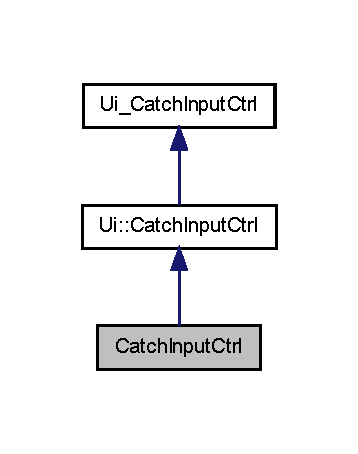
\includegraphics[width=172pt]{class_catch_input_ctrl__inherit__graph}
\end{center}
\end{figure}


Collaboration diagram for CatchInputCtrl:\nopagebreak
\begin{figure}[H]
\begin{center}
\leavevmode
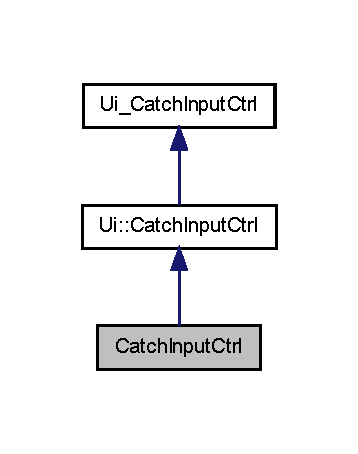
\includegraphics[width=172pt]{class_catch_input_ctrl__coll__graph}
\end{center}
\end{figure}
\subsection*{Signals}
\begin{DoxyCompactItemize}
\item 
void \hyperlink{class_catch_input_ctrl_aeb737186053f34c7b373b6d480da027d}{blockWidgetsSignals} (const bool bBlock)
\begin{DoxyCompactList}\small\item\em This is a convenience function to block/ublock signals to all the widgets contained in this control;. \item\end{DoxyCompactList}\end{DoxyCompactItemize}
\subsection*{Public Member Functions}
\begin{DoxyCompactItemize}
\item 
\hyperlink{class_catch_input_ctrl_a63859ff45f4a6b69eab7f8355f874eef}{CatchInputCtrl} (QWidget $\ast$parent=0)
\item 
\hyperlink{class_catch_input_ctrl_a4fcd5654ee8fac680e4d60643c37b1f6}{$\sim$CatchInputCtrl} ()
\item 
QDoubleSpinBox $\ast$ \hyperlink{class_catch_input_ctrl_a9e39f1a825a9e291a13b087a0daf40d9}{pDoubleSpinTotalE} ()
\begin{DoxyCompactList}\small\item\em Returns a pointer to the spinbox with the total estimated catch (weight). \item\end{DoxyCompactList}\item 
QDoubleSpinBox $\ast$ \hyperlink{class_catch_input_ctrl_a7865c365c32bb490fd8e3666c0655680}{pDoubleSpinTotalC} ()
\begin{DoxyCompactList}\small\item\em Returns a pointer to the spinbox with the total calculated catch (weight). \item\end{DoxyCompactList}\item 
QComboBox $\ast$ \hyperlink{class_catch_input_ctrl_abdbba402a6fdea21753d1ea86e4171cc}{pCmbWeightUnits} ()
\begin{DoxyCompactList}\small\item\em Returns a pointer to the combobox, with the units for the total catch. \item\end{DoxyCompactList}\item 
QDoubleSpinBox $\ast$ \hyperlink{class_catch_input_ctrl_ae79037c9816c55c8861236bd729e8022}{pDoubleSpinNoBoxesE} ()
\begin{DoxyCompactList}\small\item\em Returns a pointer to the double spinbox, with the estimated number of boxes. \item\end{DoxyCompactList}\item 
QDoubleSpinBox $\ast$ \hyperlink{class_catch_input_ctrl_aa9e7192b483cf04b02ae050210882471}{pDoubleSpinNoBoxesC} ()
\item 
QDoubleSpinBox $\ast$ \hyperlink{class_catch_input_ctrl_ac97f9a25eea77708eb3e17557a1dc698}{pDoubleSpinWeightBox} ()
\begin{DoxyCompactList}\small\item\em Returns a pointer to the double spinbox, with the calculated number of boxes. \item\end{DoxyCompactList}\item 
QComboBox $\ast$ \hyperlink{class_catch_input_ctrl_a767ffbab2894cd923ae35b762f4fae15}{pCmbBoxUnits} ()
\begin{DoxyCompactList}\small\item\em Returns a pointer to the combobox, with the units for the catch per box. \item\end{DoxyCompactList}\item 
QSpinBox $\ast$ \hyperlink{class_catch_input_ctrl_ac7e047e40d963ca82dd71e0813127a96}{pSpinUnitsE} ()
\begin{DoxyCompactList}\small\item\em Returns a pointer to the spinbox with the estimated number of catch units. \item\end{DoxyCompactList}\item 
QSpinBox $\ast$ \hyperlink{class_catch_input_ctrl_a4b4b5a8471aa3708fd2a6f142a6e325e}{pSpinUnitsC} ()
\begin{DoxyCompactList}\small\item\em Returns a pointer to the spinbox with the calculated number of catch units. \item\end{DoxyCompactList}\item 
QDoubleSpinBox $\ast$ \hyperlink{class_catch_input_ctrl_a585254c2356f7b2f0702cf1bf737950b}{pDoubleSpinWeightUnit} ()
\begin{DoxyCompactList}\small\item\em Returns a pointer to the double spinbox with the weight per unit. \item\end{DoxyCompactList}\item 
QComboBox $\ast$ \hyperlink{class_catch_input_ctrl_aee2f7b3e7ce82dbae88bea6735cefbe3}{pCmbUnitUnits} ()
\begin{DoxyCompactList}\small\item\em Returns a pointer to the combobox, with the units for the catch per unit. \item\end{DoxyCompactList}\end{DoxyCompactItemize}
\subsection*{Private Slots}
\begin{DoxyCompactItemize}
\item 
void \hyperlink{class_catch_input_ctrl_a84bac89a8b1731e8690859a0648b0f38}{adjustTotalWeightFromUnits} (int val)
\begin{DoxyCompactList}\small\item\em Adjust total weight from Units. \item\end{DoxyCompactList}\item 
void \hyperlink{class_catch_input_ctrl_af01aa84307b7bada61058771cfbac1a7}{adjustTotalWeightFromUnits} (double val)
\begin{DoxyCompactList}\small\item\em Adjust total weight from Unit Weight. \item\end{DoxyCompactList}\item 
void \hyperlink{class_catch_input_ctrl_ad524224bfc56dadce27bf72defa7ef32}{adjustTotalWeightFromNoBoxes} (double val)
\begin{DoxyCompactList}\small\item\em Adjust total weight from number of boxes. \item\end{DoxyCompactList}\item 
void \hyperlink{class_catch_input_ctrl_ac1ff61d816c6f708c176977c6b3b1e7b}{adjustTotalWeightFromBoxWeight} (double val)
\begin{DoxyCompactList}\small\item\em Adjust total weight from box weight. \item\end{DoxyCompactList}\item 
void \hyperlink{class_catch_input_ctrl_a05540b0a70693d26822081024ffec3b5}{onWeightUnitChange} (QString \hyperlink{catchinputctrl_8cpp_a40a45457a52d3c046f5b9322005ba5c5}{strUnits})
\item 
void \hyperlink{class_catch_input_ctrl_a39da14ffeffa2571fc437079debfae2f}{onUnitsUnitChange} (QString \hyperlink{catchinputctrl_8cpp_a40a45457a52d3c046f5b9322005ba5c5}{strUnits})
\item 
void \hyperlink{class_catch_input_ctrl_ad8cf089d6a877ba0471fdaf9bcaaea03}{onBoxUnitChange} (QString \hyperlink{catchinputctrl_8cpp_a40a45457a52d3c046f5b9322005ba5c5}{strUnits})
\item 
void \hyperlink{class_catch_input_ctrl_ab8e1629f9e58b12262a146f58d9309fe}{updateWeightLabel} (QString strNew)
\begin{DoxyCompactList}\small\item\em Update weight tab title. \item\end{DoxyCompactList}\item 
void \hyperlink{class_catch_input_ctrl_a0fe6e21b361de7336a2cdca8be6edb75}{onBlockWidgetsSignals} (const bool bBlock)
\end{DoxyCompactItemize}
\subsection*{Private Member Functions}
\begin{DoxyCompactItemize}
\item 
bool \hyperlink{class_catch_input_ctrl_aace7d148d134c4725f3c5aea597ea7c1}{checkUnits} (QComboBox $\ast$cmb)
\begin{DoxyCompactList}\small\item\em Check Units. \item\end{DoxyCompactList}\end{DoxyCompactItemize}


\subsection{Detailed Description}
Custom Input Control class. This control standardizes the input of catch in a UI composed of column tabs; Each tab corresponds to a different method of inputing catch, and totals are updated in the case of catch composed by a binomio (for instance unit and weight); In this way, we hope to achieve a user friendly UI that allow us to collect as much information as possible and at the same time provide some kind of validation for the user; n.b.: at this moment, unit conversions are not supported and therefore the units of the total and of the other pages have to match, in order to benefit from the calculations! 

\subsection{Constructor \& Destructor Documentation}
\hypertarget{class_catch_input_ctrl_a63859ff45f4a6b69eab7f8355f874eef}{
\index{CatchInputCtrl@{CatchInputCtrl}!CatchInputCtrl@{CatchInputCtrl}}
\index{CatchInputCtrl@{CatchInputCtrl}!CatchInputCtrl@{CatchInputCtrl}}
\subsubsection[{CatchInputCtrl}]{\setlength{\rightskip}{0pt plus 5cm}CatchInputCtrl::CatchInputCtrl (
\begin{DoxyParamCaption}
\item[{QWidget $\ast$}]{ parent = {\ttfamily 0}}
\end{DoxyParamCaption}
)}}
\label{class_catch_input_ctrl_a63859ff45f4a6b69eab7f8355f874eef}


Here is the call graph for this function:\nopagebreak
\begin{figure}[H]
\begin{center}
\leavevmode
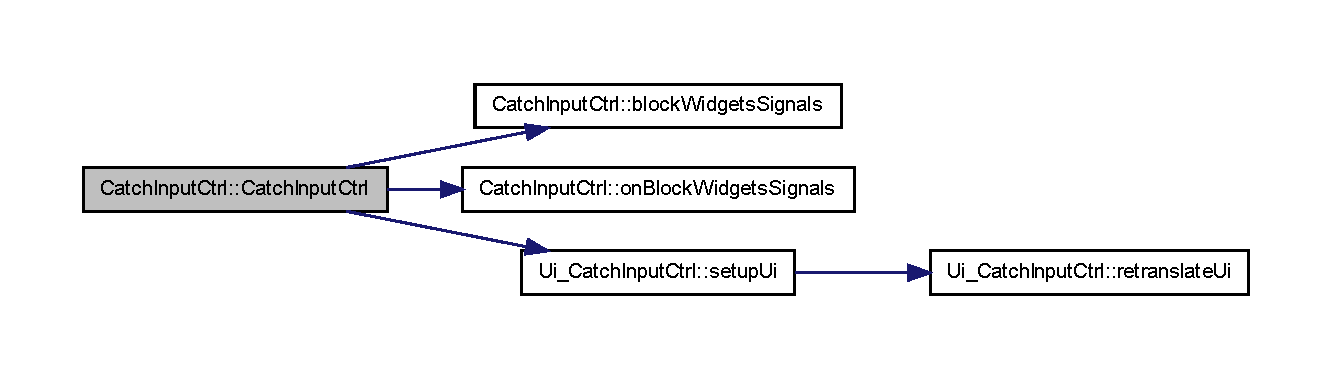
\includegraphics[width=400pt]{class_catch_input_ctrl_a63859ff45f4a6b69eab7f8355f874eef_cgraph}
\end{center}
\end{figure}


\hypertarget{class_catch_input_ctrl_a4fcd5654ee8fac680e4d60643c37b1f6}{
\index{CatchInputCtrl@{CatchInputCtrl}!$\sim$CatchInputCtrl@{$\sim$CatchInputCtrl}}
\index{$\sim$CatchInputCtrl@{$\sim$CatchInputCtrl}!CatchInputCtrl@{CatchInputCtrl}}
\subsubsection[{$\sim$CatchInputCtrl}]{\setlength{\rightskip}{0pt plus 5cm}CatchInputCtrl::$\sim$CatchInputCtrl (
\begin{DoxyParamCaption}
{}
\end{DoxyParamCaption}
)}}
\label{class_catch_input_ctrl_a4fcd5654ee8fac680e4d60643c37b1f6}


\subsection{Member Function Documentation}
\hypertarget{class_catch_input_ctrl_ac1ff61d816c6f708c176977c6b3b1e7b}{
\index{CatchInputCtrl@{CatchInputCtrl}!adjustTotalWeightFromBoxWeight@{adjustTotalWeightFromBoxWeight}}
\index{adjustTotalWeightFromBoxWeight@{adjustTotalWeightFromBoxWeight}!CatchInputCtrl@{CatchInputCtrl}}
\subsubsection[{adjustTotalWeightFromBoxWeight}]{\setlength{\rightskip}{0pt plus 5cm}void CatchInputCtrl::adjustTotalWeightFromBoxWeight (
\begin{DoxyParamCaption}
\item[{double}]{ val}
\end{DoxyParamCaption}
)\hspace{0.3cm}{\ttfamily  \mbox{[}private, slot\mbox{]}}}}
\label{class_catch_input_ctrl_ac1ff61d816c6f708c176977c6b3b1e7b}


Adjust total weight from box weight. 

Slot triggered by a box weight change, that performs the total weight calculation 
\begin{DoxyParams}{Parameters}
{\em val} & box weight \\
\hline
\end{DoxyParams}
\begin{DoxySeeAlso}{See also}
\hyperlink{class_catch_input_ctrl_a84bac89a8b1731e8690859a0648b0f38}{adjustTotalWeightFromUnits(int val)}, \hyperlink{class_catch_input_ctrl_af01aa84307b7bada61058771cfbac1a7}{adjustTotalWeightFromUnits(double val)}, \hyperlink{class_catch_input_ctrl_af01aa84307b7bada61058771cfbac1a7}{adjustTotalWeightFromUnits(double val)},\hyperlink{class_catch_input_ctrl_ad524224bfc56dadce27bf72defa7ef32}{adjustTotalWeightFromNoBoxes(double val)} 
\end{DoxySeeAlso}


Here is the call graph for this function:\nopagebreak
\begin{figure}[H]
\begin{center}
\leavevmode
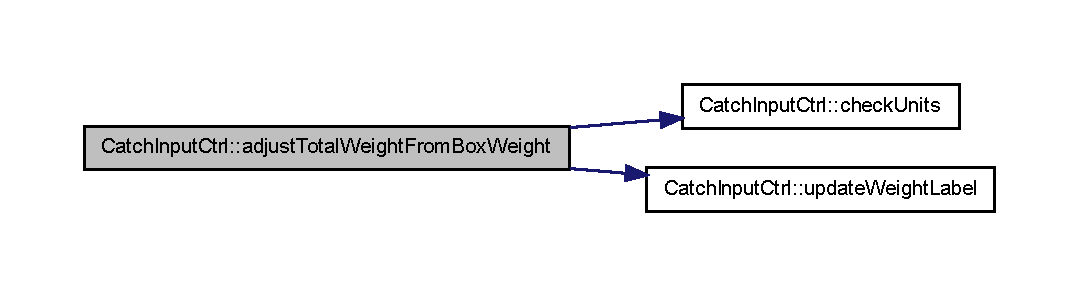
\includegraphics[width=400pt]{class_catch_input_ctrl_ac1ff61d816c6f708c176977c6b3b1e7b_cgraph}
\end{center}
\end{figure}


\hypertarget{class_catch_input_ctrl_ad524224bfc56dadce27bf72defa7ef32}{
\index{CatchInputCtrl@{CatchInputCtrl}!adjustTotalWeightFromNoBoxes@{adjustTotalWeightFromNoBoxes}}
\index{adjustTotalWeightFromNoBoxes@{adjustTotalWeightFromNoBoxes}!CatchInputCtrl@{CatchInputCtrl}}
\subsubsection[{adjustTotalWeightFromNoBoxes}]{\setlength{\rightskip}{0pt plus 5cm}void CatchInputCtrl::adjustTotalWeightFromNoBoxes (
\begin{DoxyParamCaption}
\item[{double}]{ val}
\end{DoxyParamCaption}
)\hspace{0.3cm}{\ttfamily  \mbox{[}private, slot\mbox{]}}}}
\label{class_catch_input_ctrl_ad524224bfc56dadce27bf72defa7ef32}


Adjust total weight from number of boxes. 

Slot triggered by a number of boxes change, that performs the total weight calculation 
\begin{DoxyParams}{Parameters}
{\em val} & number of boxes (as a double, so we can consider for instance half box) \\
\hline
\end{DoxyParams}
\begin{DoxySeeAlso}{See also}
\hyperlink{class_catch_input_ctrl_a84bac89a8b1731e8690859a0648b0f38}{adjustTotalWeightFromUnits(int val)}, \hyperlink{class_catch_input_ctrl_af01aa84307b7bada61058771cfbac1a7}{adjustTotalWeightFromUnits(double val)}, \hyperlink{class_catch_input_ctrl_af01aa84307b7bada61058771cfbac1a7}{adjustTotalWeightFromUnits(double val)},\hyperlink{class_catch_input_ctrl_ac1ff61d816c6f708c176977c6b3b1e7b}{adjustTotalWeightFromBoxWeight(double val)} 
\end{DoxySeeAlso}


Here is the call graph for this function:\nopagebreak
\begin{figure}[H]
\begin{center}
\leavevmode
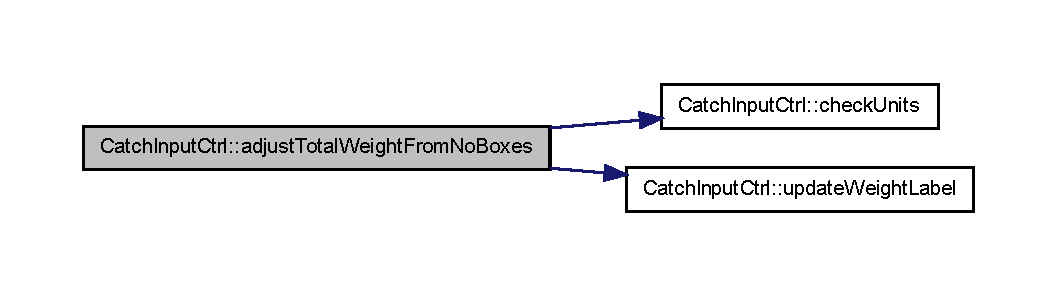
\includegraphics[width=400pt]{class_catch_input_ctrl_ad524224bfc56dadce27bf72defa7ef32_cgraph}
\end{center}
\end{figure}


\hypertarget{class_catch_input_ctrl_a84bac89a8b1731e8690859a0648b0f38}{
\index{CatchInputCtrl@{CatchInputCtrl}!adjustTotalWeightFromUnits@{adjustTotalWeightFromUnits}}
\index{adjustTotalWeightFromUnits@{adjustTotalWeightFromUnits}!CatchInputCtrl@{CatchInputCtrl}}
\subsubsection[{adjustTotalWeightFromUnits}]{\setlength{\rightskip}{0pt plus 5cm}void CatchInputCtrl::adjustTotalWeightFromUnits (
\begin{DoxyParamCaption}
\item[{int}]{ val}
\end{DoxyParamCaption}
)\hspace{0.3cm}{\ttfamily  \mbox{[}private, slot\mbox{]}}}}
\label{class_catch_input_ctrl_a84bac89a8b1731e8690859a0648b0f38}


Adjust total weight from Units. 

Slot triggered by a unit change, that performs the total weight calculation 
\begin{DoxyParams}{Parameters}
{\em val} & number of units \\
\hline
\end{DoxyParams}
\begin{DoxySeeAlso}{See also}
\hyperlink{class_catch_input_ctrl_af01aa84307b7bada61058771cfbac1a7}{adjustTotalWeightFromUnits(double val)}, \hyperlink{class_catch_input_ctrl_af01aa84307b7bada61058771cfbac1a7}{adjustTotalWeightFromUnits(double val)}, \hyperlink{class_catch_input_ctrl_ad524224bfc56dadce27bf72defa7ef32}{adjustTotalWeightFromNoBoxes(double val)},\hyperlink{class_catch_input_ctrl_ac1ff61d816c6f708c176977c6b3b1e7b}{adjustTotalWeightFromBoxWeight(double val)} 
\end{DoxySeeAlso}


Here is the call graph for this function:\nopagebreak
\begin{figure}[H]
\begin{center}
\leavevmode
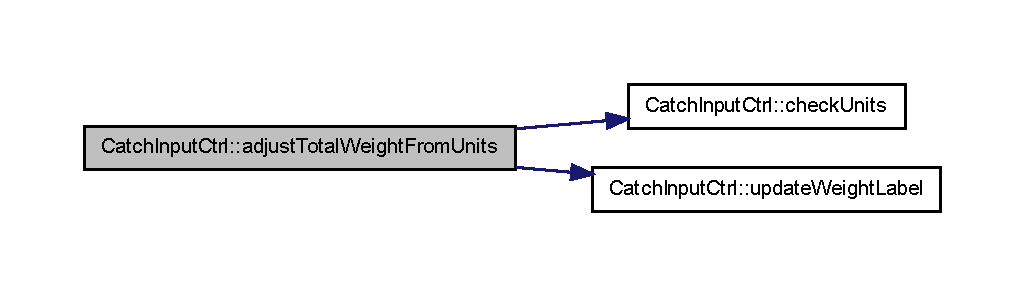
\includegraphics[width=400pt]{class_catch_input_ctrl_a84bac89a8b1731e8690859a0648b0f38_cgraph}
\end{center}
\end{figure}


\hypertarget{class_catch_input_ctrl_af01aa84307b7bada61058771cfbac1a7}{
\index{CatchInputCtrl@{CatchInputCtrl}!adjustTotalWeightFromUnits@{adjustTotalWeightFromUnits}}
\index{adjustTotalWeightFromUnits@{adjustTotalWeightFromUnits}!CatchInputCtrl@{CatchInputCtrl}}
\subsubsection[{adjustTotalWeightFromUnits}]{\setlength{\rightskip}{0pt plus 5cm}void CatchInputCtrl::adjustTotalWeightFromUnits (
\begin{DoxyParamCaption}
\item[{double}]{ val}
\end{DoxyParamCaption}
)\hspace{0.3cm}{\ttfamily  \mbox{[}private, slot\mbox{]}}}}
\label{class_catch_input_ctrl_af01aa84307b7bada61058771cfbac1a7}


Adjust total weight from Unit Weight. 

Slot triggered by a unit weight change, that performs the total weight calculation 
\begin{DoxyParams}{Parameters}
{\em val} & weight per unit \\
\hline
\end{DoxyParams}
\begin{DoxySeeAlso}{See also}
\hyperlink{class_catch_input_ctrl_a84bac89a8b1731e8690859a0648b0f38}{adjustTotalWeightFromUnits(int val)}, \hyperlink{class_catch_input_ctrl_af01aa84307b7bada61058771cfbac1a7}{adjustTotalWeightFromUnits(double val)}, \hyperlink{class_catch_input_ctrl_ad524224bfc56dadce27bf72defa7ef32}{adjustTotalWeightFromNoBoxes(double val)},\hyperlink{class_catch_input_ctrl_ac1ff61d816c6f708c176977c6b3b1e7b}{adjustTotalWeightFromBoxWeight(double val)} 
\end{DoxySeeAlso}


Here is the call graph for this function:\nopagebreak
\begin{figure}[H]
\begin{center}
\leavevmode
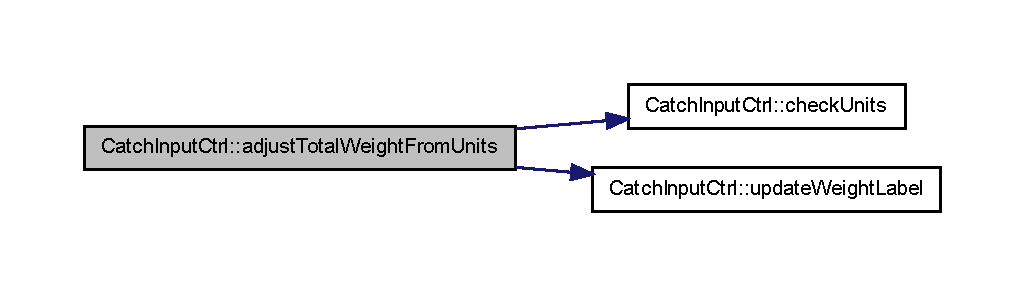
\includegraphics[width=400pt]{class_catch_input_ctrl_af01aa84307b7bada61058771cfbac1a7_cgraph}
\end{center}
\end{figure}


\hypertarget{class_catch_input_ctrl_aeb737186053f34c7b373b6d480da027d}{
\index{CatchInputCtrl@{CatchInputCtrl}!blockWidgetsSignals@{blockWidgetsSignals}}
\index{blockWidgetsSignals@{blockWidgetsSignals}!CatchInputCtrl@{CatchInputCtrl}}
\subsubsection[{blockWidgetsSignals}]{\setlength{\rightskip}{0pt plus 5cm}void CatchInputCtrl::blockWidgetsSignals (
\begin{DoxyParamCaption}
\item[{const bool}]{ bBlock}
\end{DoxyParamCaption}
)\hspace{0.3cm}{\ttfamily  \mbox{[}signal\mbox{]}}}}
\label{class_catch_input_ctrl_aeb737186053f34c7b373b6d480da027d}


This is a convenience function to block/ublock signals to all the widgets contained in this control;. 



Here is the caller graph for this function:\nopagebreak
\begin{figure}[H]
\begin{center}
\leavevmode
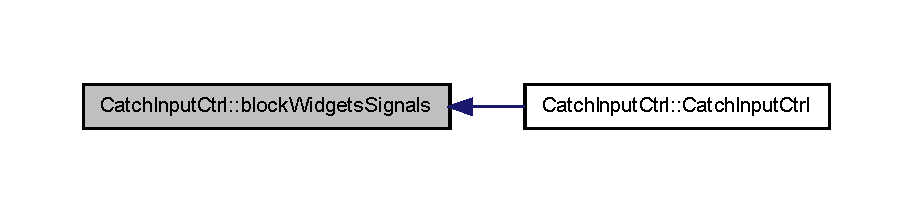
\includegraphics[width=400pt]{class_catch_input_ctrl_aeb737186053f34c7b373b6d480da027d_icgraph}
\end{center}
\end{figure}


\hypertarget{class_catch_input_ctrl_aace7d148d134c4725f3c5aea597ea7c1}{
\index{CatchInputCtrl@{CatchInputCtrl}!checkUnits@{checkUnits}}
\index{checkUnits@{checkUnits}!CatchInputCtrl@{CatchInputCtrl}}
\subsubsection[{checkUnits}]{\setlength{\rightskip}{0pt plus 5cm}bool CatchInputCtrl::checkUnits (
\begin{DoxyParamCaption}
\item[{QComboBox $\ast$}]{ cmb}
\end{DoxyParamCaption}
)\hspace{0.3cm}{\ttfamily  \mbox{[}private\mbox{]}}}}
\label{class_catch_input_ctrl_aace7d148d134c4725f3c5aea597ea7c1}


Check Units. 

Check point to ensure that the units of the current page, and the units of the total weight page match! (otherwise we cannot perform the calculation) 
\begin{DoxyParams}{Parameters}
{\em cmb} & weight combobox, so that we can retrieve the current text \\
\hline
\end{DoxyParams}


Here is the caller graph for this function:\nopagebreak
\begin{figure}[H]
\begin{center}
\leavevmode
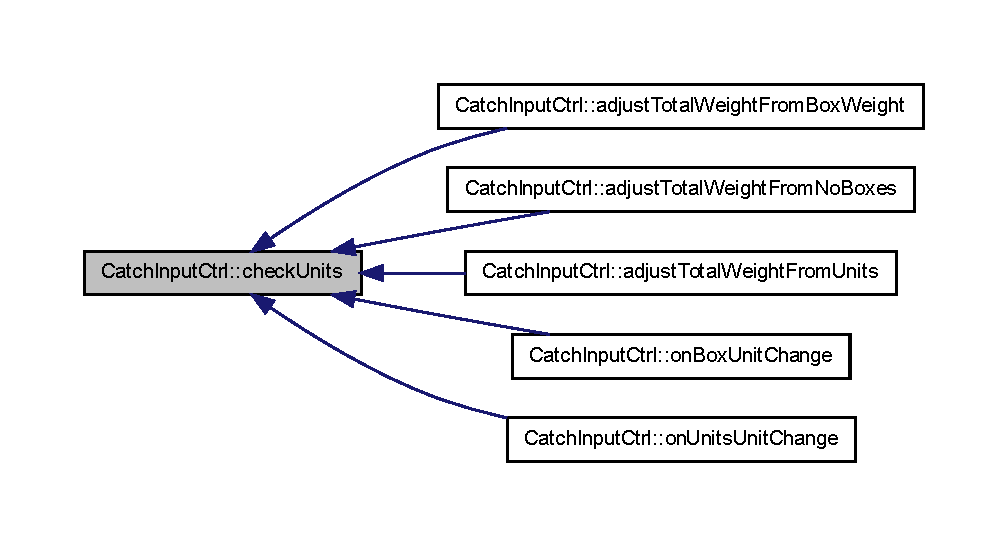
\includegraphics[width=400pt]{class_catch_input_ctrl_aace7d148d134c4725f3c5aea597ea7c1_icgraph}
\end{center}
\end{figure}


\hypertarget{class_catch_input_ctrl_a0fe6e21b361de7336a2cdca8be6edb75}{
\index{CatchInputCtrl@{CatchInputCtrl}!onBlockWidgetsSignals@{onBlockWidgetsSignals}}
\index{onBlockWidgetsSignals@{onBlockWidgetsSignals}!CatchInputCtrl@{CatchInputCtrl}}
\subsubsection[{onBlockWidgetsSignals}]{\setlength{\rightskip}{0pt plus 5cm}void CatchInputCtrl::onBlockWidgetsSignals (
\begin{DoxyParamCaption}
\item[{const bool}]{ bBlock}
\end{DoxyParamCaption}
)\hspace{0.3cm}{\ttfamily  \mbox{[}private, slot\mbox{]}}}}
\label{class_catch_input_ctrl_a0fe6e21b361de7336a2cdca8be6edb75}


Here is the caller graph for this function:\nopagebreak
\begin{figure}[H]
\begin{center}
\leavevmode
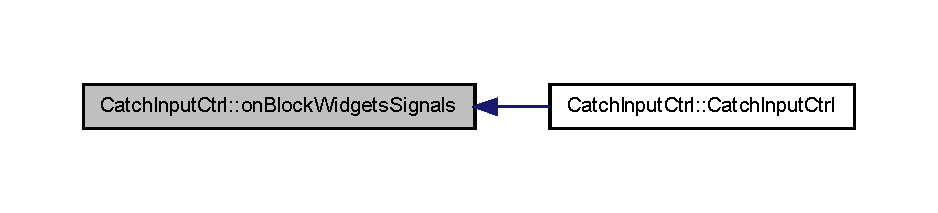
\includegraphics[width=400pt]{class_catch_input_ctrl_a0fe6e21b361de7336a2cdca8be6edb75_icgraph}
\end{center}
\end{figure}


\hypertarget{class_catch_input_ctrl_ad8cf089d6a877ba0471fdaf9bcaaea03}{
\index{CatchInputCtrl@{CatchInputCtrl}!onBoxUnitChange@{onBoxUnitChange}}
\index{onBoxUnitChange@{onBoxUnitChange}!CatchInputCtrl@{CatchInputCtrl}}
\subsubsection[{onBoxUnitChange}]{\setlength{\rightskip}{0pt plus 5cm}void CatchInputCtrl::onBoxUnitChange (
\begin{DoxyParamCaption}
\item[{QString}]{ strUnits}
\end{DoxyParamCaption}
)\hspace{0.3cm}{\ttfamily  \mbox{[}private, slot\mbox{]}}}}
\label{class_catch_input_ctrl_ad8cf089d6a877ba0471fdaf9bcaaea03}


Here is the call graph for this function:\nopagebreak
\begin{figure}[H]
\begin{center}
\leavevmode
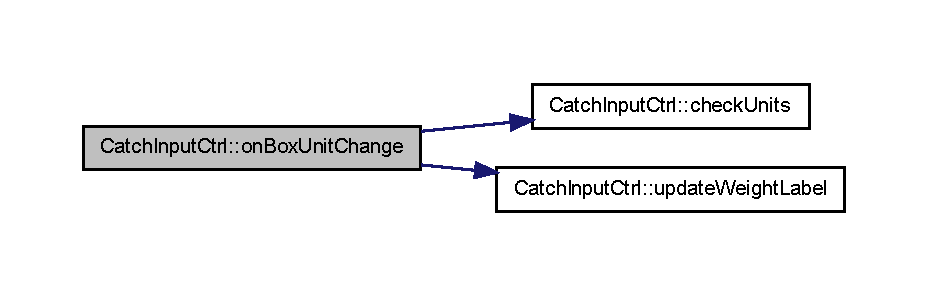
\includegraphics[width=400pt]{class_catch_input_ctrl_ad8cf089d6a877ba0471fdaf9bcaaea03_cgraph}
\end{center}
\end{figure}


\hypertarget{class_catch_input_ctrl_a39da14ffeffa2571fc437079debfae2f}{
\index{CatchInputCtrl@{CatchInputCtrl}!onUnitsUnitChange@{onUnitsUnitChange}}
\index{onUnitsUnitChange@{onUnitsUnitChange}!CatchInputCtrl@{CatchInputCtrl}}
\subsubsection[{onUnitsUnitChange}]{\setlength{\rightskip}{0pt plus 5cm}void CatchInputCtrl::onUnitsUnitChange (
\begin{DoxyParamCaption}
\item[{QString}]{ strUnits}
\end{DoxyParamCaption}
)\hspace{0.3cm}{\ttfamily  \mbox{[}private, slot\mbox{]}}}}
\label{class_catch_input_ctrl_a39da14ffeffa2571fc437079debfae2f}


Here is the call graph for this function:\nopagebreak
\begin{figure}[H]
\begin{center}
\leavevmode
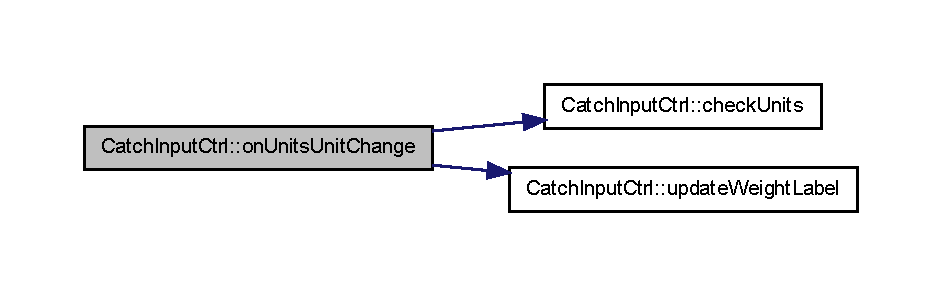
\includegraphics[width=400pt]{class_catch_input_ctrl_a39da14ffeffa2571fc437079debfae2f_cgraph}
\end{center}
\end{figure}


\hypertarget{class_catch_input_ctrl_a05540b0a70693d26822081024ffec3b5}{
\index{CatchInputCtrl@{CatchInputCtrl}!onWeightUnitChange@{onWeightUnitChange}}
\index{onWeightUnitChange@{onWeightUnitChange}!CatchInputCtrl@{CatchInputCtrl}}
\subsubsection[{onWeightUnitChange}]{\setlength{\rightskip}{0pt plus 5cm}void CatchInputCtrl::onWeightUnitChange (
\begin{DoxyParamCaption}
\item[{QString}]{ strUnits}
\end{DoxyParamCaption}
)\hspace{0.3cm}{\ttfamily  \mbox{[}private, slot\mbox{]}}}}
\label{class_catch_input_ctrl_a05540b0a70693d26822081024ffec3b5}


Here is the call graph for this function:\nopagebreak
\begin{figure}[H]
\begin{center}
\leavevmode
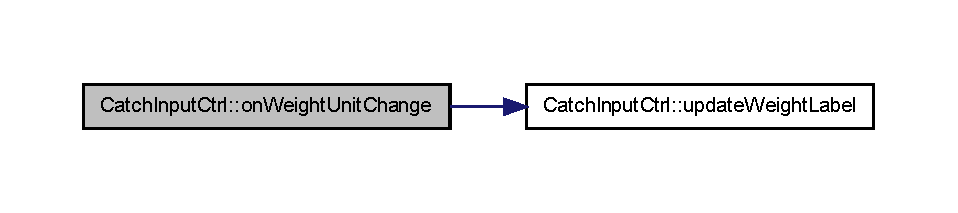
\includegraphics[width=400pt]{class_catch_input_ctrl_a05540b0a70693d26822081024ffec3b5_cgraph}
\end{center}
\end{figure}


\hypertarget{class_catch_input_ctrl_a767ffbab2894cd923ae35b762f4fae15}{
\index{CatchInputCtrl@{CatchInputCtrl}!pCmbBoxUnits@{pCmbBoxUnits}}
\index{pCmbBoxUnits@{pCmbBoxUnits}!CatchInputCtrl@{CatchInputCtrl}}
\subsubsection[{pCmbBoxUnits}]{\setlength{\rightskip}{0pt plus 5cm}QComboBox$\ast$ CatchInputCtrl::pCmbBoxUnits (
\begin{DoxyParamCaption}
{}
\end{DoxyParamCaption}
)\hspace{0.3cm}{\ttfamily  \mbox{[}inline\mbox{]}}}}
\label{class_catch_input_ctrl_a767ffbab2894cd923ae35b762f4fae15}


Returns a pointer to the combobox, with the units for the catch per box. 

\hypertarget{class_catch_input_ctrl_aee2f7b3e7ce82dbae88bea6735cefbe3}{
\index{CatchInputCtrl@{CatchInputCtrl}!pCmbUnitUnits@{pCmbUnitUnits}}
\index{pCmbUnitUnits@{pCmbUnitUnits}!CatchInputCtrl@{CatchInputCtrl}}
\subsubsection[{pCmbUnitUnits}]{\setlength{\rightskip}{0pt plus 5cm}QComboBox$\ast$ CatchInputCtrl::pCmbUnitUnits (
\begin{DoxyParamCaption}
{}
\end{DoxyParamCaption}
)\hspace{0.3cm}{\ttfamily  \mbox{[}inline\mbox{]}}}}
\label{class_catch_input_ctrl_aee2f7b3e7ce82dbae88bea6735cefbe3}


Returns a pointer to the combobox, with the units for the catch per unit. 

\hypertarget{class_catch_input_ctrl_abdbba402a6fdea21753d1ea86e4171cc}{
\index{CatchInputCtrl@{CatchInputCtrl}!pCmbWeightUnits@{pCmbWeightUnits}}
\index{pCmbWeightUnits@{pCmbWeightUnits}!CatchInputCtrl@{CatchInputCtrl}}
\subsubsection[{pCmbWeightUnits}]{\setlength{\rightskip}{0pt plus 5cm}QComboBox$\ast$ CatchInputCtrl::pCmbWeightUnits (
\begin{DoxyParamCaption}
{}
\end{DoxyParamCaption}
)\hspace{0.3cm}{\ttfamily  \mbox{[}inline\mbox{]}}}}
\label{class_catch_input_ctrl_abdbba402a6fdea21753d1ea86e4171cc}


Returns a pointer to the combobox, with the units for the total catch. 

\hypertarget{class_catch_input_ctrl_aa9e7192b483cf04b02ae050210882471}{
\index{CatchInputCtrl@{CatchInputCtrl}!pDoubleSpinNoBoxesC@{pDoubleSpinNoBoxesC}}
\index{pDoubleSpinNoBoxesC@{pDoubleSpinNoBoxesC}!CatchInputCtrl@{CatchInputCtrl}}
\subsubsection[{pDoubleSpinNoBoxesC}]{\setlength{\rightskip}{0pt plus 5cm}QDoubleSpinBox$\ast$ CatchInputCtrl::pDoubleSpinNoBoxesC (
\begin{DoxyParamCaption}
{}
\end{DoxyParamCaption}
)\hspace{0.3cm}{\ttfamily  \mbox{[}inline\mbox{]}}}}
\label{class_catch_input_ctrl_aa9e7192b483cf04b02ae050210882471}
\hypertarget{class_catch_input_ctrl_ae79037c9816c55c8861236bd729e8022}{
\index{CatchInputCtrl@{CatchInputCtrl}!pDoubleSpinNoBoxesE@{pDoubleSpinNoBoxesE}}
\index{pDoubleSpinNoBoxesE@{pDoubleSpinNoBoxesE}!CatchInputCtrl@{CatchInputCtrl}}
\subsubsection[{pDoubleSpinNoBoxesE}]{\setlength{\rightskip}{0pt plus 5cm}QDoubleSpinBox$\ast$ CatchInputCtrl::pDoubleSpinNoBoxesE (
\begin{DoxyParamCaption}
{}
\end{DoxyParamCaption}
)\hspace{0.3cm}{\ttfamily  \mbox{[}inline\mbox{]}}}}
\label{class_catch_input_ctrl_ae79037c9816c55c8861236bd729e8022}


Returns a pointer to the double spinbox, with the estimated number of boxes. 

\hypertarget{class_catch_input_ctrl_a7865c365c32bb490fd8e3666c0655680}{
\index{CatchInputCtrl@{CatchInputCtrl}!pDoubleSpinTotalC@{pDoubleSpinTotalC}}
\index{pDoubleSpinTotalC@{pDoubleSpinTotalC}!CatchInputCtrl@{CatchInputCtrl}}
\subsubsection[{pDoubleSpinTotalC}]{\setlength{\rightskip}{0pt plus 5cm}QDoubleSpinBox$\ast$ CatchInputCtrl::pDoubleSpinTotalC (
\begin{DoxyParamCaption}
{}
\end{DoxyParamCaption}
)\hspace{0.3cm}{\ttfamily  \mbox{[}inline\mbox{]}}}}
\label{class_catch_input_ctrl_a7865c365c32bb490fd8e3666c0655680}


Returns a pointer to the spinbox with the total calculated catch (weight). 

\hypertarget{class_catch_input_ctrl_a9e39f1a825a9e291a13b087a0daf40d9}{
\index{CatchInputCtrl@{CatchInputCtrl}!pDoubleSpinTotalE@{pDoubleSpinTotalE}}
\index{pDoubleSpinTotalE@{pDoubleSpinTotalE}!CatchInputCtrl@{CatchInputCtrl}}
\subsubsection[{pDoubleSpinTotalE}]{\setlength{\rightskip}{0pt plus 5cm}QDoubleSpinBox$\ast$ CatchInputCtrl::pDoubleSpinTotalE (
\begin{DoxyParamCaption}
{}
\end{DoxyParamCaption}
)\hspace{0.3cm}{\ttfamily  \mbox{[}inline\mbox{]}}}}
\label{class_catch_input_ctrl_a9e39f1a825a9e291a13b087a0daf40d9}


Returns a pointer to the spinbox with the total estimated catch (weight). 

\hypertarget{class_catch_input_ctrl_ac97f9a25eea77708eb3e17557a1dc698}{
\index{CatchInputCtrl@{CatchInputCtrl}!pDoubleSpinWeightBox@{pDoubleSpinWeightBox}}
\index{pDoubleSpinWeightBox@{pDoubleSpinWeightBox}!CatchInputCtrl@{CatchInputCtrl}}
\subsubsection[{pDoubleSpinWeightBox}]{\setlength{\rightskip}{0pt plus 5cm}QDoubleSpinBox$\ast$ CatchInputCtrl::pDoubleSpinWeightBox (
\begin{DoxyParamCaption}
{}
\end{DoxyParamCaption}
)\hspace{0.3cm}{\ttfamily  \mbox{[}inline\mbox{]}}}}
\label{class_catch_input_ctrl_ac97f9a25eea77708eb3e17557a1dc698}


Returns a pointer to the double spinbox, with the calculated number of boxes. 

Returns a pointer to the double spinbox, with the weight per box. \hypertarget{class_catch_input_ctrl_a585254c2356f7b2f0702cf1bf737950b}{
\index{CatchInputCtrl@{CatchInputCtrl}!pDoubleSpinWeightUnit@{pDoubleSpinWeightUnit}}
\index{pDoubleSpinWeightUnit@{pDoubleSpinWeightUnit}!CatchInputCtrl@{CatchInputCtrl}}
\subsubsection[{pDoubleSpinWeightUnit}]{\setlength{\rightskip}{0pt plus 5cm}QDoubleSpinBox$\ast$ CatchInputCtrl::pDoubleSpinWeightUnit (
\begin{DoxyParamCaption}
{}
\end{DoxyParamCaption}
)\hspace{0.3cm}{\ttfamily  \mbox{[}inline\mbox{]}}}}
\label{class_catch_input_ctrl_a585254c2356f7b2f0702cf1bf737950b}


Returns a pointer to the double spinbox with the weight per unit. 

\hypertarget{class_catch_input_ctrl_a4b4b5a8471aa3708fd2a6f142a6e325e}{
\index{CatchInputCtrl@{CatchInputCtrl}!pSpinUnitsC@{pSpinUnitsC}}
\index{pSpinUnitsC@{pSpinUnitsC}!CatchInputCtrl@{CatchInputCtrl}}
\subsubsection[{pSpinUnitsC}]{\setlength{\rightskip}{0pt plus 5cm}QSpinBox$\ast$ CatchInputCtrl::pSpinUnitsC (
\begin{DoxyParamCaption}
{}
\end{DoxyParamCaption}
)\hspace{0.3cm}{\ttfamily  \mbox{[}inline\mbox{]}}}}
\label{class_catch_input_ctrl_a4b4b5a8471aa3708fd2a6f142a6e325e}


Returns a pointer to the spinbox with the calculated number of catch units. 

\hypertarget{class_catch_input_ctrl_ac7e047e40d963ca82dd71e0813127a96}{
\index{CatchInputCtrl@{CatchInputCtrl}!pSpinUnitsE@{pSpinUnitsE}}
\index{pSpinUnitsE@{pSpinUnitsE}!CatchInputCtrl@{CatchInputCtrl}}
\subsubsection[{pSpinUnitsE}]{\setlength{\rightskip}{0pt plus 5cm}QSpinBox$\ast$ CatchInputCtrl::pSpinUnitsE (
\begin{DoxyParamCaption}
{}
\end{DoxyParamCaption}
)\hspace{0.3cm}{\ttfamily  \mbox{[}inline\mbox{]}}}}
\label{class_catch_input_ctrl_ac7e047e40d963ca82dd71e0813127a96}


Returns a pointer to the spinbox with the estimated number of catch units. 

\hypertarget{class_catch_input_ctrl_ab8e1629f9e58b12262a146f58d9309fe}{
\index{CatchInputCtrl@{CatchInputCtrl}!updateWeightLabel@{updateWeightLabel}}
\index{updateWeightLabel@{updateWeightLabel}!CatchInputCtrl@{CatchInputCtrl}}
\subsubsection[{updateWeightLabel}]{\setlength{\rightskip}{0pt plus 5cm}void CatchInputCtrl::updateWeightLabel (
\begin{DoxyParamCaption}
\item[{QString}]{ strNew}
\end{DoxyParamCaption}
)\hspace{0.3cm}{\ttfamily  \mbox{[}private, slot\mbox{]}}}}
\label{class_catch_input_ctrl_ab8e1629f9e58b12262a146f58d9309fe}


Update weight tab title. 

This function generates dynamically a tab title, with a total 

Here is the caller graph for this function:\nopagebreak
\begin{figure}[H]
\begin{center}
\leavevmode
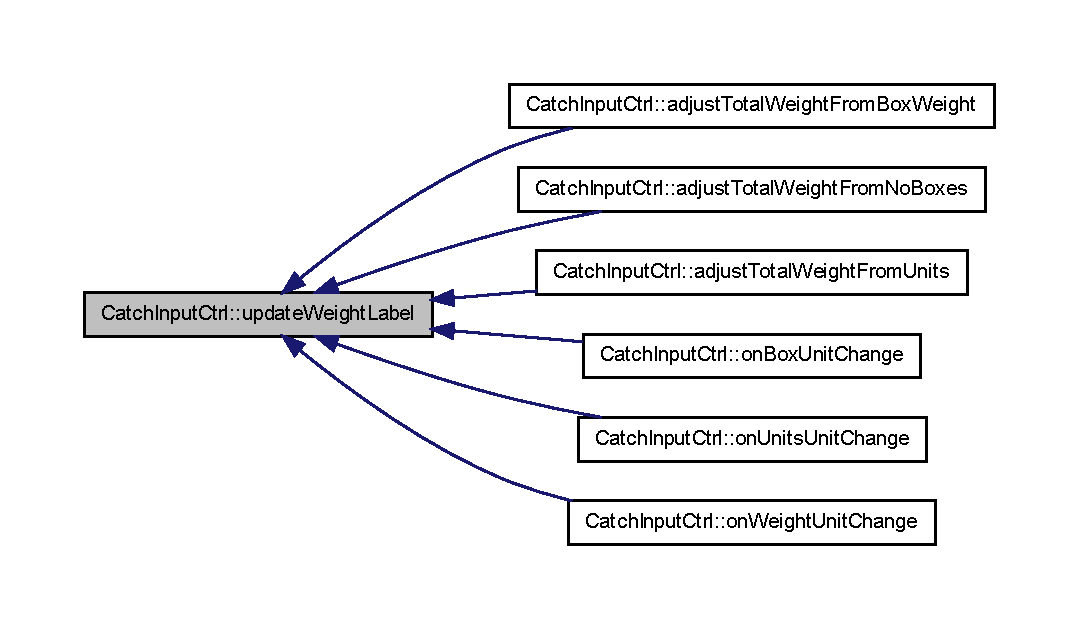
\includegraphics[width=400pt]{class_catch_input_ctrl_ab8e1629f9e58b12262a146f58d9309fe_icgraph}
\end{center}
\end{figure}




The documentation for this class was generated from the following files:\begin{DoxyCompactItemize}
\item 
CatchInputCtrl/\hyperlink{catchinputctrl_8h}{catchinputctrl.h}\item 
CatchInputCtrl/\hyperlink{catchinputctrl_8cpp}{catchinputctrl.cpp}\item 
CatchInputCtrl/GeneratedFiles/Debug/\hyperlink{_debug_2moc__catchinputctrl_8cpp}{moc\_\-catchinputctrl.cpp}\item 
CatchInputCtrl/GeneratedFiles/Release/\hyperlink{_release_2moc__catchinputctrl_8cpp}{moc\_\-catchinputctrl.cpp}\end{DoxyCompactItemize}

\hypertarget{class_ui_1_1_catch_input_ctrl}{
\section{Ui::CatchInputCtrl Class Reference}
\label{class_ui_1_1_catch_input_ctrl}\index{Ui::CatchInputCtrl@{Ui::CatchInputCtrl}}
}


{\ttfamily \#include $<$ui\_\-catchinputfrm.h$>$}



Inheritance diagram for Ui::CatchInputCtrl:\nopagebreak
\begin{figure}[H]
\begin{center}
\leavevmode
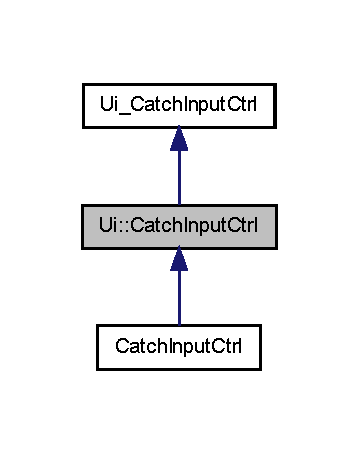
\includegraphics[width=172pt]{class_ui_1_1_catch_input_ctrl__inherit__graph}
\end{center}
\end{figure}


Collaboration diagram for Ui::CatchInputCtrl:\nopagebreak
\begin{figure}[H]
\begin{center}
\leavevmode
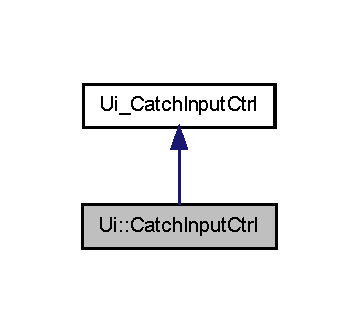
\includegraphics[width=172pt]{class_ui_1_1_catch_input_ctrl__coll__graph}
\end{center}
\end{figure}


The documentation for this class was generated from the following file:\begin{DoxyCompactItemize}
\item 
CatchInputCtrl/GeneratedFiles/\hyperlink{ui__catchinputfrm_8h}{ui\_\-catchinputfrm.h}\end{DoxyCompactItemize}

\hypertarget{class_catch_input_ctrl_plugin}{
\section{CatchInputCtrlPlugin Class Reference}
\label{class_catch_input_ctrl_plugin}\index{CatchInputCtrlPlugin@{CatchInputCtrlPlugin}}
}


Plugin Class.  




{\ttfamily \#include $<$catchinputctrlplugin.h$>$}

\subsection*{Public Member Functions}
\begin{DoxyCompactItemize}
\item 
\hyperlink{class_catch_input_ctrl_plugin_a1834eb9eccaa2a7b4966eed509cae7bc}{CatchInputCtrlPlugin} (QObject $\ast$parent=0)
\item 
bool \hyperlink{class_catch_input_ctrl_plugin_a1a2c7380b2d904e4878d3f7bbe7f57d6}{isContainer} () const 
\item 
bool \hyperlink{class_catch_input_ctrl_plugin_aa61345caf7253e2f205a43507f43bde6}{isInitialized} () const 
\item 
QIcon \hyperlink{class_catch_input_ctrl_plugin_adc87f03a325e9c981762a883f12aed51}{icon} () const 
\begin{DoxyCompactList}\small\item\em Icon for this plugin;. \item\end{DoxyCompactList}\item 
QString \hyperlink{class_catch_input_ctrl_plugin_a1916108461bf1a08e37c8fe9069e980c}{domXml} () const 
\item 
QString \hyperlink{class_catch_input_ctrl_plugin_a2e9a0a0ec3a9484f2c7bd3475519aafc}{group} () const 
\begin{DoxyCompactList}\small\item\em Group for this plugin, in the Designer;. \item\end{DoxyCompactList}\item 
QString \hyperlink{class_catch_input_ctrl_plugin_a18718a7ff1e4614583361193cef4c218}{includeFile} () const 
\begin{DoxyCompactList}\small\item\em Include file for the plugin;. \item\end{DoxyCompactList}\item 
QString \hyperlink{class_catch_input_ctrl_plugin_aa238f9656fda644bf61f061b9eb296fb}{name} () const 
\begin{DoxyCompactList}\small\item\em Plugin name;. \item\end{DoxyCompactList}\item 
QString \hyperlink{class_catch_input_ctrl_plugin_a66815b8920b223db303bfde2bc9997f1}{toolTip} () const 
\begin{DoxyCompactList}\small\item\em Plugin tooltip;. \item\end{DoxyCompactList}\item 
QString \hyperlink{class_catch_input_ctrl_plugin_adb249d9957a8144c004f939efd5c6f42}{whatsThis} () const 
\begin{DoxyCompactList}\small\item\em Plugin whatsThis;. \item\end{DoxyCompactList}\item 
QWidget $\ast$ \hyperlink{class_catch_input_ctrl_plugin_a6327b5527f7124b0093f0b8d3030d77c}{createWidget} (QWidget $\ast$parent)
\begin{DoxyCompactList}\small\item\em Method that instantiates the catchinputctrl class (and therefore the control);. \item\end{DoxyCompactList}\item 
void \hyperlink{class_catch_input_ctrl_plugin_af074e338042ad431cced1f03ad42d9b9}{initialize} (QDesignerFormEditorInterface $\ast$core)
\end{DoxyCompactItemize}
\subsection*{Private Attributes}
\begin{DoxyCompactItemize}
\item 
bool \hyperlink{class_catch_input_ctrl_plugin_ac3600bda2c53684e37b1890b9371f720}{initialized}
\end{DoxyCompactItemize}


\subsection{Detailed Description}
Plugin Class. This is the class exposed as a plugin; it is ihneritated from QDesignerCustomWidgetInterface, which is an custom class for Qt designer plugins. 

\subsection{Constructor \& Destructor Documentation}
\hypertarget{class_catch_input_ctrl_plugin_a1834eb9eccaa2a7b4966eed509cae7bc}{
\index{CatchInputCtrlPlugin@{CatchInputCtrlPlugin}!CatchInputCtrlPlugin@{CatchInputCtrlPlugin}}
\index{CatchInputCtrlPlugin@{CatchInputCtrlPlugin}!CatchInputCtrlPlugin@{CatchInputCtrlPlugin}}
\subsubsection[{CatchInputCtrlPlugin}]{\setlength{\rightskip}{0pt plus 5cm}CatchInputCtrlPlugin::CatchInputCtrlPlugin (
\begin{DoxyParamCaption}
\item[{QObject $\ast$}]{ parent = {\ttfamily 0}}
\end{DoxyParamCaption}
)}}
\label{class_catch_input_ctrl_plugin_a1834eb9eccaa2a7b4966eed509cae7bc}


\subsection{Member Function Documentation}
\hypertarget{class_catch_input_ctrl_plugin_a6327b5527f7124b0093f0b8d3030d77c}{
\index{CatchInputCtrlPlugin@{CatchInputCtrlPlugin}!createWidget@{createWidget}}
\index{createWidget@{createWidget}!CatchInputCtrlPlugin@{CatchInputCtrlPlugin}}
\subsubsection[{createWidget}]{\setlength{\rightskip}{0pt plus 5cm}QWidget $\ast$ CatchInputCtrlPlugin::createWidget (
\begin{DoxyParamCaption}
\item[{QWidget $\ast$}]{ parent}
\end{DoxyParamCaption}
)}}
\label{class_catch_input_ctrl_plugin_a6327b5527f7124b0093f0b8d3030d77c}


Method that instantiates the catchinputctrl class (and therefore the control);. 

\hypertarget{class_catch_input_ctrl_plugin_a1916108461bf1a08e37c8fe9069e980c}{
\index{CatchInputCtrlPlugin@{CatchInputCtrlPlugin}!domXml@{domXml}}
\index{domXml@{domXml}!CatchInputCtrlPlugin@{CatchInputCtrlPlugin}}
\subsubsection[{domXml}]{\setlength{\rightskip}{0pt plus 5cm}QString CatchInputCtrlPlugin::domXml (
\begin{DoxyParamCaption}
{}
\end{DoxyParamCaption}
) const}}
\label{class_catch_input_ctrl_plugin_a1916108461bf1a08e37c8fe9069e980c}
\hypertarget{class_catch_input_ctrl_plugin_a2e9a0a0ec3a9484f2c7bd3475519aafc}{
\index{CatchInputCtrlPlugin@{CatchInputCtrlPlugin}!group@{group}}
\index{group@{group}!CatchInputCtrlPlugin@{CatchInputCtrlPlugin}}
\subsubsection[{group}]{\setlength{\rightskip}{0pt plus 5cm}QString CatchInputCtrlPlugin::group (
\begin{DoxyParamCaption}
{}
\end{DoxyParamCaption}
) const}}
\label{class_catch_input_ctrl_plugin_a2e9a0a0ec3a9484f2c7bd3475519aafc}


Group for this plugin, in the Designer;. 

\hypertarget{class_catch_input_ctrl_plugin_adc87f03a325e9c981762a883f12aed51}{
\index{CatchInputCtrlPlugin@{CatchInputCtrlPlugin}!icon@{icon}}
\index{icon@{icon}!CatchInputCtrlPlugin@{CatchInputCtrlPlugin}}
\subsubsection[{icon}]{\setlength{\rightskip}{0pt plus 5cm}QIcon CatchInputCtrlPlugin::icon (
\begin{DoxyParamCaption}
{}
\end{DoxyParamCaption}
) const}}
\label{class_catch_input_ctrl_plugin_adc87f03a325e9c981762a883f12aed51}


Icon for this plugin;. 

\hypertarget{class_catch_input_ctrl_plugin_a18718a7ff1e4614583361193cef4c218}{
\index{CatchInputCtrlPlugin@{CatchInputCtrlPlugin}!includeFile@{includeFile}}
\index{includeFile@{includeFile}!CatchInputCtrlPlugin@{CatchInputCtrlPlugin}}
\subsubsection[{includeFile}]{\setlength{\rightskip}{0pt plus 5cm}QString CatchInputCtrlPlugin::includeFile (
\begin{DoxyParamCaption}
{}
\end{DoxyParamCaption}
) const}}
\label{class_catch_input_ctrl_plugin_a18718a7ff1e4614583361193cef4c218}


Include file for the plugin;. 

\hypertarget{class_catch_input_ctrl_plugin_af074e338042ad431cced1f03ad42d9b9}{
\index{CatchInputCtrlPlugin@{CatchInputCtrlPlugin}!initialize@{initialize}}
\index{initialize@{initialize}!CatchInputCtrlPlugin@{CatchInputCtrlPlugin}}
\subsubsection[{initialize}]{\setlength{\rightskip}{0pt plus 5cm}void CatchInputCtrlPlugin::initialize (
\begin{DoxyParamCaption}
\item[{QDesignerFormEditorInterface $\ast$}]{ core}
\end{DoxyParamCaption}
)}}
\label{class_catch_input_ctrl_plugin_af074e338042ad431cced1f03ad42d9b9}
\hypertarget{class_catch_input_ctrl_plugin_a1a2c7380b2d904e4878d3f7bbe7f57d6}{
\index{CatchInputCtrlPlugin@{CatchInputCtrlPlugin}!isContainer@{isContainer}}
\index{isContainer@{isContainer}!CatchInputCtrlPlugin@{CatchInputCtrlPlugin}}
\subsubsection[{isContainer}]{\setlength{\rightskip}{0pt plus 5cm}bool CatchInputCtrlPlugin::isContainer (
\begin{DoxyParamCaption}
{}
\end{DoxyParamCaption}
) const}}
\label{class_catch_input_ctrl_plugin_a1a2c7380b2d904e4878d3f7bbe7f57d6}
\hypertarget{class_catch_input_ctrl_plugin_aa61345caf7253e2f205a43507f43bde6}{
\index{CatchInputCtrlPlugin@{CatchInputCtrlPlugin}!isInitialized@{isInitialized}}
\index{isInitialized@{isInitialized}!CatchInputCtrlPlugin@{CatchInputCtrlPlugin}}
\subsubsection[{isInitialized}]{\setlength{\rightskip}{0pt plus 5cm}bool CatchInputCtrlPlugin::isInitialized (
\begin{DoxyParamCaption}
{}
\end{DoxyParamCaption}
) const}}
\label{class_catch_input_ctrl_plugin_aa61345caf7253e2f205a43507f43bde6}
\hypertarget{class_catch_input_ctrl_plugin_aa238f9656fda644bf61f061b9eb296fb}{
\index{CatchInputCtrlPlugin@{CatchInputCtrlPlugin}!name@{name}}
\index{name@{name}!CatchInputCtrlPlugin@{CatchInputCtrlPlugin}}
\subsubsection[{name}]{\setlength{\rightskip}{0pt plus 5cm}QString CatchInputCtrlPlugin::name (
\begin{DoxyParamCaption}
{}
\end{DoxyParamCaption}
) const}}
\label{class_catch_input_ctrl_plugin_aa238f9656fda644bf61f061b9eb296fb}


Plugin name;. 

\hypertarget{class_catch_input_ctrl_plugin_a66815b8920b223db303bfde2bc9997f1}{
\index{CatchInputCtrlPlugin@{CatchInputCtrlPlugin}!toolTip@{toolTip}}
\index{toolTip@{toolTip}!CatchInputCtrlPlugin@{CatchInputCtrlPlugin}}
\subsubsection[{toolTip}]{\setlength{\rightskip}{0pt plus 5cm}QString CatchInputCtrlPlugin::toolTip (
\begin{DoxyParamCaption}
{}
\end{DoxyParamCaption}
) const}}
\label{class_catch_input_ctrl_plugin_a66815b8920b223db303bfde2bc9997f1}


Plugin tooltip;. 

\hypertarget{class_catch_input_ctrl_plugin_adb249d9957a8144c004f939efd5c6f42}{
\index{CatchInputCtrlPlugin@{CatchInputCtrlPlugin}!whatsThis@{whatsThis}}
\index{whatsThis@{whatsThis}!CatchInputCtrlPlugin@{CatchInputCtrlPlugin}}
\subsubsection[{whatsThis}]{\setlength{\rightskip}{0pt plus 5cm}QString CatchInputCtrlPlugin::whatsThis (
\begin{DoxyParamCaption}
{}
\end{DoxyParamCaption}
) const}}
\label{class_catch_input_ctrl_plugin_adb249d9957a8144c004f939efd5c6f42}


Plugin whatsThis;. 



\subsection{Member Data Documentation}
\hypertarget{class_catch_input_ctrl_plugin_ac3600bda2c53684e37b1890b9371f720}{
\index{CatchInputCtrlPlugin@{CatchInputCtrlPlugin}!initialized@{initialized}}
\index{initialized@{initialized}!CatchInputCtrlPlugin@{CatchInputCtrlPlugin}}
\subsubsection[{initialized}]{\setlength{\rightskip}{0pt plus 5cm}bool {\bf CatchInputCtrlPlugin::initialized}\hspace{0.3cm}{\ttfamily  \mbox{[}private\mbox{]}}}}
\label{class_catch_input_ctrl_plugin_ac3600bda2c53684e37b1890b9371f720}


The documentation for this class was generated from the following files:\begin{DoxyCompactItemize}
\item 
CatchInputCtrl/\hyperlink{catchinputctrlplugin_8h}{catchinputctrlplugin.h}\item 
CatchInputCtrl/\hyperlink{catchinputctrlplugin_8cpp}{catchinputctrlplugin.cpp}\end{DoxyCompactItemize}

\hypertarget{class_ui___catch_input_ctrl}{
\section{Ui\_\-CatchInputCtrl Class Reference}
\label{class_ui___catch_input_ctrl}\index{Ui\_\-CatchInputCtrl@{Ui\_\-CatchInputCtrl}}
}


{\ttfamily \#include $<$ui\_\-catchinputfrm.h$>$}



Inheritance diagram for Ui\_\-CatchInputCtrl:\nopagebreak
\begin{figure}[H]
\begin{center}
\leavevmode
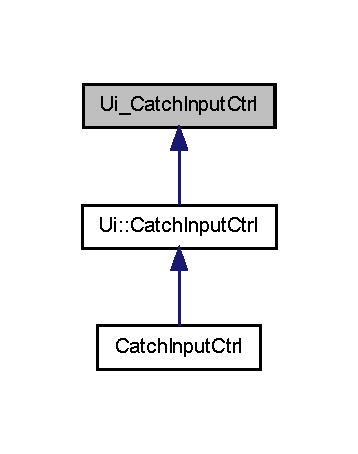
\includegraphics[width=172pt]{class_ui___catch_input_ctrl__inherit__graph}
\end{center}
\end{figure}
\subsection*{Public Member Functions}
\begin{DoxyCompactItemize}
\item 
void \hyperlink{class_ui___catch_input_ctrl_aac3148ff222d28ab8911bf1dd9f2a7d5}{setupUi} (QWidget $\ast$\hyperlink{class_catch_input_ctrl}{CatchInputCtrl})
\item 
void \hyperlink{class_ui___catch_input_ctrl_a25736584c7fc37974b9de94ed919df6d}{retranslateUi} (QWidget $\ast$\hyperlink{class_catch_input_ctrl}{CatchInputCtrl})
\end{DoxyCompactItemize}
\subsection*{Public Attributes}
\begin{DoxyCompactItemize}
\item 
QVBoxLayout $\ast$ \hyperlink{class_ui___catch_input_ctrl_a9561b6529376d26e0ccb20cc6c14b250}{verticalLayout}
\item 
QToolBox $\ast$ \hyperlink{class_ui___catch_input_ctrl_a400cc2815d260b0d5a2002e0f3930624}{toolBox}
\item 
QWidget $\ast$ \hyperlink{class_ui___catch_input_ctrl_a9537a8bca138a8be186818857687c60b}{pageWeight}
\item 
QGridLayout $\ast$ \hyperlink{class_ui___catch_input_ctrl_a9100755b8172afb9af709d31006d35ca}{gridLayout\_\-3}
\item 
QLabel $\ast$ \hyperlink{class_ui___catch_input_ctrl_a749bd3c4cfc56b285f3433a29fbd7f4f}{label}
\item 
QLabel $\ast$ \hyperlink{class_ui___catch_input_ctrl_afc6d97fb8770eb2a9b8c12e0c8b3e8ab}{label\_\-2}
\item 
QLabel $\ast$ \hyperlink{class_ui___catch_input_ctrl_a7dfdb06aa7352b97b76fd6c46d1bf409}{label\_\-3}
\item 
QDoubleSpinBox $\ast$ \hyperlink{class_ui___catch_input_ctrl_a78f71e94d3f0fa1afb22097a90f9c32c}{doubleSpinTotalE}
\item 
QDoubleSpinBox $\ast$ \hyperlink{class_ui___catch_input_ctrl_aff17e56983eb8a28a43bee32c447cbc9}{doubleSpinTotalC}
\item 
QComboBox $\ast$ \hyperlink{class_ui___catch_input_ctrl_ac34db8d516987f86bab23d83c406fd8c}{cmbWeightUnits}
\item 
QWidget $\ast$ \hyperlink{class_ui___catch_input_ctrl_ae3a68f52213e0032bdc63a85d983e78f}{pageBoxes}
\item 
QGridLayout $\ast$ \hyperlink{class_ui___catch_input_ctrl_af1f917ff0f390f088908fd7f1d476b98}{gridLayout\_\-2}
\item 
QLabel $\ast$ \hyperlink{class_ui___catch_input_ctrl_a5a44fb5339f63d2428392e01c5218679}{label\_\-4}
\item 
QLabel $\ast$ \hyperlink{class_ui___catch_input_ctrl_a360c2f2b5fa15408bcb206816a0ea865}{label\_\-5}
\item 
QLabel $\ast$ \hyperlink{class_ui___catch_input_ctrl_a022e39dbe397e76af5c51d2c7c17934b}{label\_\-6}
\item 
QLabel $\ast$ \hyperlink{class_ui___catch_input_ctrl_a2b0edb00030f14ac2c6fee7de386b5d9}{label\_\-7}
\item 
QDoubleSpinBox $\ast$ \hyperlink{class_ui___catch_input_ctrl_aa9fa8f4049a06445c3abbc8291ffe0b3}{doubleSpinNoBoxesE}
\item 
QDoubleSpinBox $\ast$ \hyperlink{class_ui___catch_input_ctrl_a08cd9de7440362184d996c4a693f1738}{doubleSpinNoBoxesC}
\item 
QDoubleSpinBox $\ast$ \hyperlink{class_ui___catch_input_ctrl_aca5b5c50124d550c442508bf5c871b37}{doubleSpinWeightBox}
\item 
QComboBox $\ast$ \hyperlink{class_ui___catch_input_ctrl_ae8f1e20253a8b76bd62f6149b758c13e}{cmbBoxUnits}
\item 
QWidget $\ast$ \hyperlink{class_ui___catch_input_ctrl_ad4d3f4960d555a6730cb0351d284d7e3}{pageUnits}
\item 
QGridLayout $\ast$ \hyperlink{class_ui___catch_input_ctrl_abce8903ef568863906ac33edc67a8f25}{gridLayout}
\item 
QLabel $\ast$ \hyperlink{class_ui___catch_input_ctrl_a916da0c8449e61b9f1c073ff0c2e155c}{label\_\-8}
\item 
QLabel $\ast$ \hyperlink{class_ui___catch_input_ctrl_aa16e8593fe0e150db98bd00e8960554f}{label\_\-9}
\item 
QLabel $\ast$ \hyperlink{class_ui___catch_input_ctrl_afeb1c5fca99de7c2ce25627d5bd712a1}{label\_\-10}
\item 
QLabel $\ast$ \hyperlink{class_ui___catch_input_ctrl_a27c801d7bf9931f63ac93ead50253d45}{label\_\-11}
\item 
QSpinBox $\ast$ \hyperlink{class_ui___catch_input_ctrl_af103c39dda2853d367ade43e1819b817}{spinUnitsE}
\item 
QSpinBox $\ast$ \hyperlink{class_ui___catch_input_ctrl_a6c04044f260cf28a4b66e0e9eeda55da}{spinUnitsC}
\item 
QDoubleSpinBox $\ast$ \hyperlink{class_ui___catch_input_ctrl_a3a85d92aac141bde03e7842eb58e3973}{doubleSpinWeightUnit}
\item 
QComboBox $\ast$ \hyperlink{class_ui___catch_input_ctrl_a02f01f7a03385a0502fbd2d6d557e9a4}{cmbUnitUnits}
\end{DoxyCompactItemize}


\subsection{Member Function Documentation}
\hypertarget{class_ui___catch_input_ctrl_a25736584c7fc37974b9de94ed919df6d}{
\index{Ui\_\-CatchInputCtrl@{Ui\_\-CatchInputCtrl}!retranslateUi@{retranslateUi}}
\index{retranslateUi@{retranslateUi}!Ui_CatchInputCtrl@{Ui\_\-CatchInputCtrl}}
\subsubsection[{retranslateUi}]{\setlength{\rightskip}{0pt plus 5cm}void Ui\_\-CatchInputCtrl::retranslateUi (
\begin{DoxyParamCaption}
\item[{QWidget $\ast$}]{ CatchInputCtrl}
\end{DoxyParamCaption}
)\hspace{0.3cm}{\ttfamily  \mbox{[}inline\mbox{]}}}}
\label{class_ui___catch_input_ctrl_a25736584c7fc37974b9de94ed919df6d}


Here is the caller graph for this function:\nopagebreak
\begin{figure}[H]
\begin{center}
\leavevmode
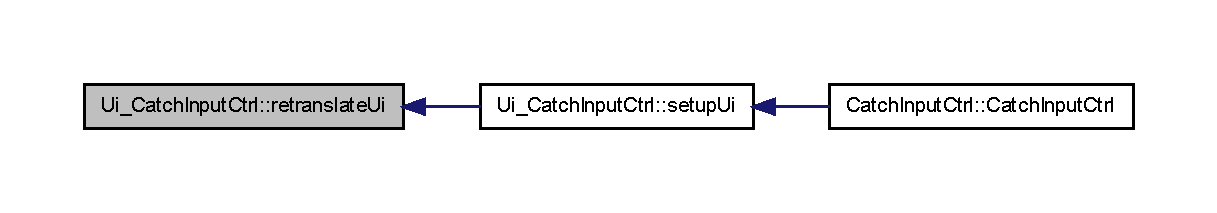
\includegraphics[width=400pt]{class_ui___catch_input_ctrl_a25736584c7fc37974b9de94ed919df6d_icgraph}
\end{center}
\end{figure}


\hypertarget{class_ui___catch_input_ctrl_aac3148ff222d28ab8911bf1dd9f2a7d5}{
\index{Ui\_\-CatchInputCtrl@{Ui\_\-CatchInputCtrl}!setupUi@{setupUi}}
\index{setupUi@{setupUi}!Ui_CatchInputCtrl@{Ui\_\-CatchInputCtrl}}
\subsubsection[{setupUi}]{\setlength{\rightskip}{0pt plus 5cm}void Ui\_\-CatchInputCtrl::setupUi (
\begin{DoxyParamCaption}
\item[{QWidget $\ast$}]{ CatchInputCtrl}
\end{DoxyParamCaption}
)\hspace{0.3cm}{\ttfamily  \mbox{[}inline\mbox{]}}}}
\label{class_ui___catch_input_ctrl_aac3148ff222d28ab8911bf1dd9f2a7d5}


Here is the call graph for this function:\nopagebreak
\begin{figure}[H]
\begin{center}
\leavevmode
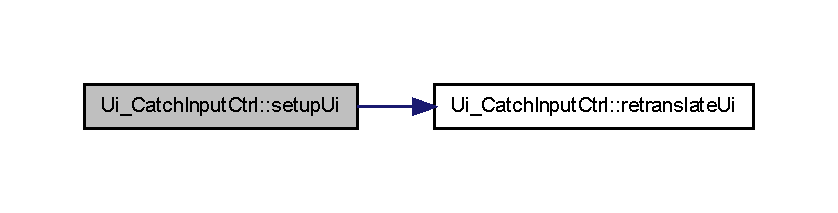
\includegraphics[width=400pt]{class_ui___catch_input_ctrl_aac3148ff222d28ab8911bf1dd9f2a7d5_cgraph}
\end{center}
\end{figure}




Here is the caller graph for this function:\nopagebreak
\begin{figure}[H]
\begin{center}
\leavevmode
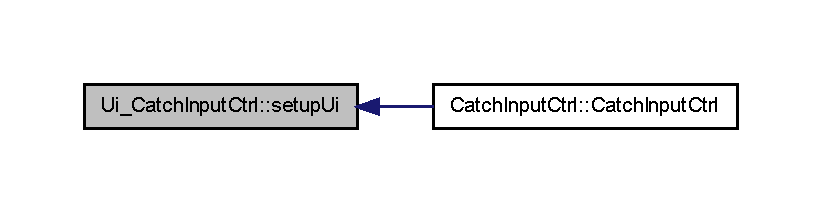
\includegraphics[width=394pt]{class_ui___catch_input_ctrl_aac3148ff222d28ab8911bf1dd9f2a7d5_icgraph}
\end{center}
\end{figure}




\subsection{Member Data Documentation}
\hypertarget{class_ui___catch_input_ctrl_ae8f1e20253a8b76bd62f6149b758c13e}{
\index{Ui\_\-CatchInputCtrl@{Ui\_\-CatchInputCtrl}!cmbBoxUnits@{cmbBoxUnits}}
\index{cmbBoxUnits@{cmbBoxUnits}!Ui_CatchInputCtrl@{Ui\_\-CatchInputCtrl}}
\subsubsection[{cmbBoxUnits}]{\setlength{\rightskip}{0pt plus 5cm}QComboBox$\ast$ {\bf Ui\_\-CatchInputCtrl::cmbBoxUnits}}}
\label{class_ui___catch_input_ctrl_ae8f1e20253a8b76bd62f6149b758c13e}
\hypertarget{class_ui___catch_input_ctrl_a02f01f7a03385a0502fbd2d6d557e9a4}{
\index{Ui\_\-CatchInputCtrl@{Ui\_\-CatchInputCtrl}!cmbUnitUnits@{cmbUnitUnits}}
\index{cmbUnitUnits@{cmbUnitUnits}!Ui_CatchInputCtrl@{Ui\_\-CatchInputCtrl}}
\subsubsection[{cmbUnitUnits}]{\setlength{\rightskip}{0pt plus 5cm}QComboBox$\ast$ {\bf Ui\_\-CatchInputCtrl::cmbUnitUnits}}}
\label{class_ui___catch_input_ctrl_a02f01f7a03385a0502fbd2d6d557e9a4}
\hypertarget{class_ui___catch_input_ctrl_ac34db8d516987f86bab23d83c406fd8c}{
\index{Ui\_\-CatchInputCtrl@{Ui\_\-CatchInputCtrl}!cmbWeightUnits@{cmbWeightUnits}}
\index{cmbWeightUnits@{cmbWeightUnits}!Ui_CatchInputCtrl@{Ui\_\-CatchInputCtrl}}
\subsubsection[{cmbWeightUnits}]{\setlength{\rightskip}{0pt plus 5cm}QComboBox$\ast$ {\bf Ui\_\-CatchInputCtrl::cmbWeightUnits}}}
\label{class_ui___catch_input_ctrl_ac34db8d516987f86bab23d83c406fd8c}
\hypertarget{class_ui___catch_input_ctrl_a08cd9de7440362184d996c4a693f1738}{
\index{Ui\_\-CatchInputCtrl@{Ui\_\-CatchInputCtrl}!doubleSpinNoBoxesC@{doubleSpinNoBoxesC}}
\index{doubleSpinNoBoxesC@{doubleSpinNoBoxesC}!Ui_CatchInputCtrl@{Ui\_\-CatchInputCtrl}}
\subsubsection[{doubleSpinNoBoxesC}]{\setlength{\rightskip}{0pt plus 5cm}QDoubleSpinBox$\ast$ {\bf Ui\_\-CatchInputCtrl::doubleSpinNoBoxesC}}}
\label{class_ui___catch_input_ctrl_a08cd9de7440362184d996c4a693f1738}
\hypertarget{class_ui___catch_input_ctrl_aa9fa8f4049a06445c3abbc8291ffe0b3}{
\index{Ui\_\-CatchInputCtrl@{Ui\_\-CatchInputCtrl}!doubleSpinNoBoxesE@{doubleSpinNoBoxesE}}
\index{doubleSpinNoBoxesE@{doubleSpinNoBoxesE}!Ui_CatchInputCtrl@{Ui\_\-CatchInputCtrl}}
\subsubsection[{doubleSpinNoBoxesE}]{\setlength{\rightskip}{0pt plus 5cm}QDoubleSpinBox$\ast$ {\bf Ui\_\-CatchInputCtrl::doubleSpinNoBoxesE}}}
\label{class_ui___catch_input_ctrl_aa9fa8f4049a06445c3abbc8291ffe0b3}
\hypertarget{class_ui___catch_input_ctrl_aff17e56983eb8a28a43bee32c447cbc9}{
\index{Ui\_\-CatchInputCtrl@{Ui\_\-CatchInputCtrl}!doubleSpinTotalC@{doubleSpinTotalC}}
\index{doubleSpinTotalC@{doubleSpinTotalC}!Ui_CatchInputCtrl@{Ui\_\-CatchInputCtrl}}
\subsubsection[{doubleSpinTotalC}]{\setlength{\rightskip}{0pt plus 5cm}QDoubleSpinBox$\ast$ {\bf Ui\_\-CatchInputCtrl::doubleSpinTotalC}}}
\label{class_ui___catch_input_ctrl_aff17e56983eb8a28a43bee32c447cbc9}
\hypertarget{class_ui___catch_input_ctrl_a78f71e94d3f0fa1afb22097a90f9c32c}{
\index{Ui\_\-CatchInputCtrl@{Ui\_\-CatchInputCtrl}!doubleSpinTotalE@{doubleSpinTotalE}}
\index{doubleSpinTotalE@{doubleSpinTotalE}!Ui_CatchInputCtrl@{Ui\_\-CatchInputCtrl}}
\subsubsection[{doubleSpinTotalE}]{\setlength{\rightskip}{0pt plus 5cm}QDoubleSpinBox$\ast$ {\bf Ui\_\-CatchInputCtrl::doubleSpinTotalE}}}
\label{class_ui___catch_input_ctrl_a78f71e94d3f0fa1afb22097a90f9c32c}
\hypertarget{class_ui___catch_input_ctrl_aca5b5c50124d550c442508bf5c871b37}{
\index{Ui\_\-CatchInputCtrl@{Ui\_\-CatchInputCtrl}!doubleSpinWeightBox@{doubleSpinWeightBox}}
\index{doubleSpinWeightBox@{doubleSpinWeightBox}!Ui_CatchInputCtrl@{Ui\_\-CatchInputCtrl}}
\subsubsection[{doubleSpinWeightBox}]{\setlength{\rightskip}{0pt plus 5cm}QDoubleSpinBox$\ast$ {\bf Ui\_\-CatchInputCtrl::doubleSpinWeightBox}}}
\label{class_ui___catch_input_ctrl_aca5b5c50124d550c442508bf5c871b37}
\hypertarget{class_ui___catch_input_ctrl_a3a85d92aac141bde03e7842eb58e3973}{
\index{Ui\_\-CatchInputCtrl@{Ui\_\-CatchInputCtrl}!doubleSpinWeightUnit@{doubleSpinWeightUnit}}
\index{doubleSpinWeightUnit@{doubleSpinWeightUnit}!Ui_CatchInputCtrl@{Ui\_\-CatchInputCtrl}}
\subsubsection[{doubleSpinWeightUnit}]{\setlength{\rightskip}{0pt plus 5cm}QDoubleSpinBox$\ast$ {\bf Ui\_\-CatchInputCtrl::doubleSpinWeightUnit}}}
\label{class_ui___catch_input_ctrl_a3a85d92aac141bde03e7842eb58e3973}
\hypertarget{class_ui___catch_input_ctrl_abce8903ef568863906ac33edc67a8f25}{
\index{Ui\_\-CatchInputCtrl@{Ui\_\-CatchInputCtrl}!gridLayout@{gridLayout}}
\index{gridLayout@{gridLayout}!Ui_CatchInputCtrl@{Ui\_\-CatchInputCtrl}}
\subsubsection[{gridLayout}]{\setlength{\rightskip}{0pt plus 5cm}QGridLayout$\ast$ {\bf Ui\_\-CatchInputCtrl::gridLayout}}}
\label{class_ui___catch_input_ctrl_abce8903ef568863906ac33edc67a8f25}
\hypertarget{class_ui___catch_input_ctrl_af1f917ff0f390f088908fd7f1d476b98}{
\index{Ui\_\-CatchInputCtrl@{Ui\_\-CatchInputCtrl}!gridLayout\_\-2@{gridLayout\_\-2}}
\index{gridLayout\_\-2@{gridLayout\_\-2}!Ui_CatchInputCtrl@{Ui\_\-CatchInputCtrl}}
\subsubsection[{gridLayout\_\-2}]{\setlength{\rightskip}{0pt plus 5cm}QGridLayout$\ast$ {\bf Ui\_\-CatchInputCtrl::gridLayout\_\-2}}}
\label{class_ui___catch_input_ctrl_af1f917ff0f390f088908fd7f1d476b98}
\hypertarget{class_ui___catch_input_ctrl_a9100755b8172afb9af709d31006d35ca}{
\index{Ui\_\-CatchInputCtrl@{Ui\_\-CatchInputCtrl}!gridLayout\_\-3@{gridLayout\_\-3}}
\index{gridLayout\_\-3@{gridLayout\_\-3}!Ui_CatchInputCtrl@{Ui\_\-CatchInputCtrl}}
\subsubsection[{gridLayout\_\-3}]{\setlength{\rightskip}{0pt plus 5cm}QGridLayout$\ast$ {\bf Ui\_\-CatchInputCtrl::gridLayout\_\-3}}}
\label{class_ui___catch_input_ctrl_a9100755b8172afb9af709d31006d35ca}
\hypertarget{class_ui___catch_input_ctrl_a749bd3c4cfc56b285f3433a29fbd7f4f}{
\index{Ui\_\-CatchInputCtrl@{Ui\_\-CatchInputCtrl}!label@{label}}
\index{label@{label}!Ui_CatchInputCtrl@{Ui\_\-CatchInputCtrl}}
\subsubsection[{label}]{\setlength{\rightskip}{0pt plus 5cm}QLabel$\ast$ {\bf Ui\_\-CatchInputCtrl::label}}}
\label{class_ui___catch_input_ctrl_a749bd3c4cfc56b285f3433a29fbd7f4f}
\hypertarget{class_ui___catch_input_ctrl_afeb1c5fca99de7c2ce25627d5bd712a1}{
\index{Ui\_\-CatchInputCtrl@{Ui\_\-CatchInputCtrl}!label\_\-10@{label\_\-10}}
\index{label\_\-10@{label\_\-10}!Ui_CatchInputCtrl@{Ui\_\-CatchInputCtrl}}
\subsubsection[{label\_\-10}]{\setlength{\rightskip}{0pt plus 5cm}QLabel$\ast$ {\bf Ui\_\-CatchInputCtrl::label\_\-10}}}
\label{class_ui___catch_input_ctrl_afeb1c5fca99de7c2ce25627d5bd712a1}
\hypertarget{class_ui___catch_input_ctrl_a27c801d7bf9931f63ac93ead50253d45}{
\index{Ui\_\-CatchInputCtrl@{Ui\_\-CatchInputCtrl}!label\_\-11@{label\_\-11}}
\index{label\_\-11@{label\_\-11}!Ui_CatchInputCtrl@{Ui\_\-CatchInputCtrl}}
\subsubsection[{label\_\-11}]{\setlength{\rightskip}{0pt plus 5cm}QLabel$\ast$ {\bf Ui\_\-CatchInputCtrl::label\_\-11}}}
\label{class_ui___catch_input_ctrl_a27c801d7bf9931f63ac93ead50253d45}
\hypertarget{class_ui___catch_input_ctrl_afc6d97fb8770eb2a9b8c12e0c8b3e8ab}{
\index{Ui\_\-CatchInputCtrl@{Ui\_\-CatchInputCtrl}!label\_\-2@{label\_\-2}}
\index{label\_\-2@{label\_\-2}!Ui_CatchInputCtrl@{Ui\_\-CatchInputCtrl}}
\subsubsection[{label\_\-2}]{\setlength{\rightskip}{0pt plus 5cm}QLabel$\ast$ {\bf Ui\_\-CatchInputCtrl::label\_\-2}}}
\label{class_ui___catch_input_ctrl_afc6d97fb8770eb2a9b8c12e0c8b3e8ab}
\hypertarget{class_ui___catch_input_ctrl_a7dfdb06aa7352b97b76fd6c46d1bf409}{
\index{Ui\_\-CatchInputCtrl@{Ui\_\-CatchInputCtrl}!label\_\-3@{label\_\-3}}
\index{label\_\-3@{label\_\-3}!Ui_CatchInputCtrl@{Ui\_\-CatchInputCtrl}}
\subsubsection[{label\_\-3}]{\setlength{\rightskip}{0pt plus 5cm}QLabel$\ast$ {\bf Ui\_\-CatchInputCtrl::label\_\-3}}}
\label{class_ui___catch_input_ctrl_a7dfdb06aa7352b97b76fd6c46d1bf409}
\hypertarget{class_ui___catch_input_ctrl_a5a44fb5339f63d2428392e01c5218679}{
\index{Ui\_\-CatchInputCtrl@{Ui\_\-CatchInputCtrl}!label\_\-4@{label\_\-4}}
\index{label\_\-4@{label\_\-4}!Ui_CatchInputCtrl@{Ui\_\-CatchInputCtrl}}
\subsubsection[{label\_\-4}]{\setlength{\rightskip}{0pt plus 5cm}QLabel$\ast$ {\bf Ui\_\-CatchInputCtrl::label\_\-4}}}
\label{class_ui___catch_input_ctrl_a5a44fb5339f63d2428392e01c5218679}
\hypertarget{class_ui___catch_input_ctrl_a360c2f2b5fa15408bcb206816a0ea865}{
\index{Ui\_\-CatchInputCtrl@{Ui\_\-CatchInputCtrl}!label\_\-5@{label\_\-5}}
\index{label\_\-5@{label\_\-5}!Ui_CatchInputCtrl@{Ui\_\-CatchInputCtrl}}
\subsubsection[{label\_\-5}]{\setlength{\rightskip}{0pt plus 5cm}QLabel$\ast$ {\bf Ui\_\-CatchInputCtrl::label\_\-5}}}
\label{class_ui___catch_input_ctrl_a360c2f2b5fa15408bcb206816a0ea865}
\hypertarget{class_ui___catch_input_ctrl_a022e39dbe397e76af5c51d2c7c17934b}{
\index{Ui\_\-CatchInputCtrl@{Ui\_\-CatchInputCtrl}!label\_\-6@{label\_\-6}}
\index{label\_\-6@{label\_\-6}!Ui_CatchInputCtrl@{Ui\_\-CatchInputCtrl}}
\subsubsection[{label\_\-6}]{\setlength{\rightskip}{0pt plus 5cm}QLabel$\ast$ {\bf Ui\_\-CatchInputCtrl::label\_\-6}}}
\label{class_ui___catch_input_ctrl_a022e39dbe397e76af5c51d2c7c17934b}
\hypertarget{class_ui___catch_input_ctrl_a2b0edb00030f14ac2c6fee7de386b5d9}{
\index{Ui\_\-CatchInputCtrl@{Ui\_\-CatchInputCtrl}!label\_\-7@{label\_\-7}}
\index{label\_\-7@{label\_\-7}!Ui_CatchInputCtrl@{Ui\_\-CatchInputCtrl}}
\subsubsection[{label\_\-7}]{\setlength{\rightskip}{0pt plus 5cm}QLabel$\ast$ {\bf Ui\_\-CatchInputCtrl::label\_\-7}}}
\label{class_ui___catch_input_ctrl_a2b0edb00030f14ac2c6fee7de386b5d9}
\hypertarget{class_ui___catch_input_ctrl_a916da0c8449e61b9f1c073ff0c2e155c}{
\index{Ui\_\-CatchInputCtrl@{Ui\_\-CatchInputCtrl}!label\_\-8@{label\_\-8}}
\index{label\_\-8@{label\_\-8}!Ui_CatchInputCtrl@{Ui\_\-CatchInputCtrl}}
\subsubsection[{label\_\-8}]{\setlength{\rightskip}{0pt plus 5cm}QLabel$\ast$ {\bf Ui\_\-CatchInputCtrl::label\_\-8}}}
\label{class_ui___catch_input_ctrl_a916da0c8449e61b9f1c073ff0c2e155c}
\hypertarget{class_ui___catch_input_ctrl_aa16e8593fe0e150db98bd00e8960554f}{
\index{Ui\_\-CatchInputCtrl@{Ui\_\-CatchInputCtrl}!label\_\-9@{label\_\-9}}
\index{label\_\-9@{label\_\-9}!Ui_CatchInputCtrl@{Ui\_\-CatchInputCtrl}}
\subsubsection[{label\_\-9}]{\setlength{\rightskip}{0pt plus 5cm}QLabel$\ast$ {\bf Ui\_\-CatchInputCtrl::label\_\-9}}}
\label{class_ui___catch_input_ctrl_aa16e8593fe0e150db98bd00e8960554f}
\hypertarget{class_ui___catch_input_ctrl_ae3a68f52213e0032bdc63a85d983e78f}{
\index{Ui\_\-CatchInputCtrl@{Ui\_\-CatchInputCtrl}!pageBoxes@{pageBoxes}}
\index{pageBoxes@{pageBoxes}!Ui_CatchInputCtrl@{Ui\_\-CatchInputCtrl}}
\subsubsection[{pageBoxes}]{\setlength{\rightskip}{0pt plus 5cm}QWidget$\ast$ {\bf Ui\_\-CatchInputCtrl::pageBoxes}}}
\label{class_ui___catch_input_ctrl_ae3a68f52213e0032bdc63a85d983e78f}
\hypertarget{class_ui___catch_input_ctrl_ad4d3f4960d555a6730cb0351d284d7e3}{
\index{Ui\_\-CatchInputCtrl@{Ui\_\-CatchInputCtrl}!pageUnits@{pageUnits}}
\index{pageUnits@{pageUnits}!Ui_CatchInputCtrl@{Ui\_\-CatchInputCtrl}}
\subsubsection[{pageUnits}]{\setlength{\rightskip}{0pt plus 5cm}QWidget$\ast$ {\bf Ui\_\-CatchInputCtrl::pageUnits}}}
\label{class_ui___catch_input_ctrl_ad4d3f4960d555a6730cb0351d284d7e3}
\hypertarget{class_ui___catch_input_ctrl_a9537a8bca138a8be186818857687c60b}{
\index{Ui\_\-CatchInputCtrl@{Ui\_\-CatchInputCtrl}!pageWeight@{pageWeight}}
\index{pageWeight@{pageWeight}!Ui_CatchInputCtrl@{Ui\_\-CatchInputCtrl}}
\subsubsection[{pageWeight}]{\setlength{\rightskip}{0pt plus 5cm}QWidget$\ast$ {\bf Ui\_\-CatchInputCtrl::pageWeight}}}
\label{class_ui___catch_input_ctrl_a9537a8bca138a8be186818857687c60b}
\hypertarget{class_ui___catch_input_ctrl_a6c04044f260cf28a4b66e0e9eeda55da}{
\index{Ui\_\-CatchInputCtrl@{Ui\_\-CatchInputCtrl}!spinUnitsC@{spinUnitsC}}
\index{spinUnitsC@{spinUnitsC}!Ui_CatchInputCtrl@{Ui\_\-CatchInputCtrl}}
\subsubsection[{spinUnitsC}]{\setlength{\rightskip}{0pt plus 5cm}QSpinBox$\ast$ {\bf Ui\_\-CatchInputCtrl::spinUnitsC}}}
\label{class_ui___catch_input_ctrl_a6c04044f260cf28a4b66e0e9eeda55da}
\hypertarget{class_ui___catch_input_ctrl_af103c39dda2853d367ade43e1819b817}{
\index{Ui\_\-CatchInputCtrl@{Ui\_\-CatchInputCtrl}!spinUnitsE@{spinUnitsE}}
\index{spinUnitsE@{spinUnitsE}!Ui_CatchInputCtrl@{Ui\_\-CatchInputCtrl}}
\subsubsection[{spinUnitsE}]{\setlength{\rightskip}{0pt plus 5cm}QSpinBox$\ast$ {\bf Ui\_\-CatchInputCtrl::spinUnitsE}}}
\label{class_ui___catch_input_ctrl_af103c39dda2853d367ade43e1819b817}
\hypertarget{class_ui___catch_input_ctrl_a400cc2815d260b0d5a2002e0f3930624}{
\index{Ui\_\-CatchInputCtrl@{Ui\_\-CatchInputCtrl}!toolBox@{toolBox}}
\index{toolBox@{toolBox}!Ui_CatchInputCtrl@{Ui\_\-CatchInputCtrl}}
\subsubsection[{toolBox}]{\setlength{\rightskip}{0pt plus 5cm}QToolBox$\ast$ {\bf Ui\_\-CatchInputCtrl::toolBox}}}
\label{class_ui___catch_input_ctrl_a400cc2815d260b0d5a2002e0f3930624}
\hypertarget{class_ui___catch_input_ctrl_a9561b6529376d26e0ccb20cc6c14b250}{
\index{Ui\_\-CatchInputCtrl@{Ui\_\-CatchInputCtrl}!verticalLayout@{verticalLayout}}
\index{verticalLayout@{verticalLayout}!Ui_CatchInputCtrl@{Ui\_\-CatchInputCtrl}}
\subsubsection[{verticalLayout}]{\setlength{\rightskip}{0pt plus 5cm}QVBoxLayout$\ast$ {\bf Ui\_\-CatchInputCtrl::verticalLayout}}}
\label{class_ui___catch_input_ctrl_a9561b6529376d26e0ccb20cc6c14b250}


The documentation for this class was generated from the following file:\begin{DoxyCompactItemize}
\item 
CatchInputCtrl/GeneratedFiles/\hyperlink{ui__catchinputfrm_8h}{ui\_\-catchinputfrm.h}\end{DoxyCompactItemize}

\chapter{File Documentation}
\hypertarget{catchinputctrl_8cpp}{
\section{CatchInputCtrl/catchinputctrl.cpp File Reference}
\label{catchinputctrl_8cpp}\index{CatchInputCtrl/catchinputctrl.cpp@{CatchInputCtrl/catchinputctrl.cpp}}
}
{\ttfamily \#include \char`\"{}catchinputctrl.h\char`\"{}}\par
Include dependency graph for catchinputctrl.cpp:\nopagebreak
\begin{figure}[H]
\begin{center}
\leavevmode
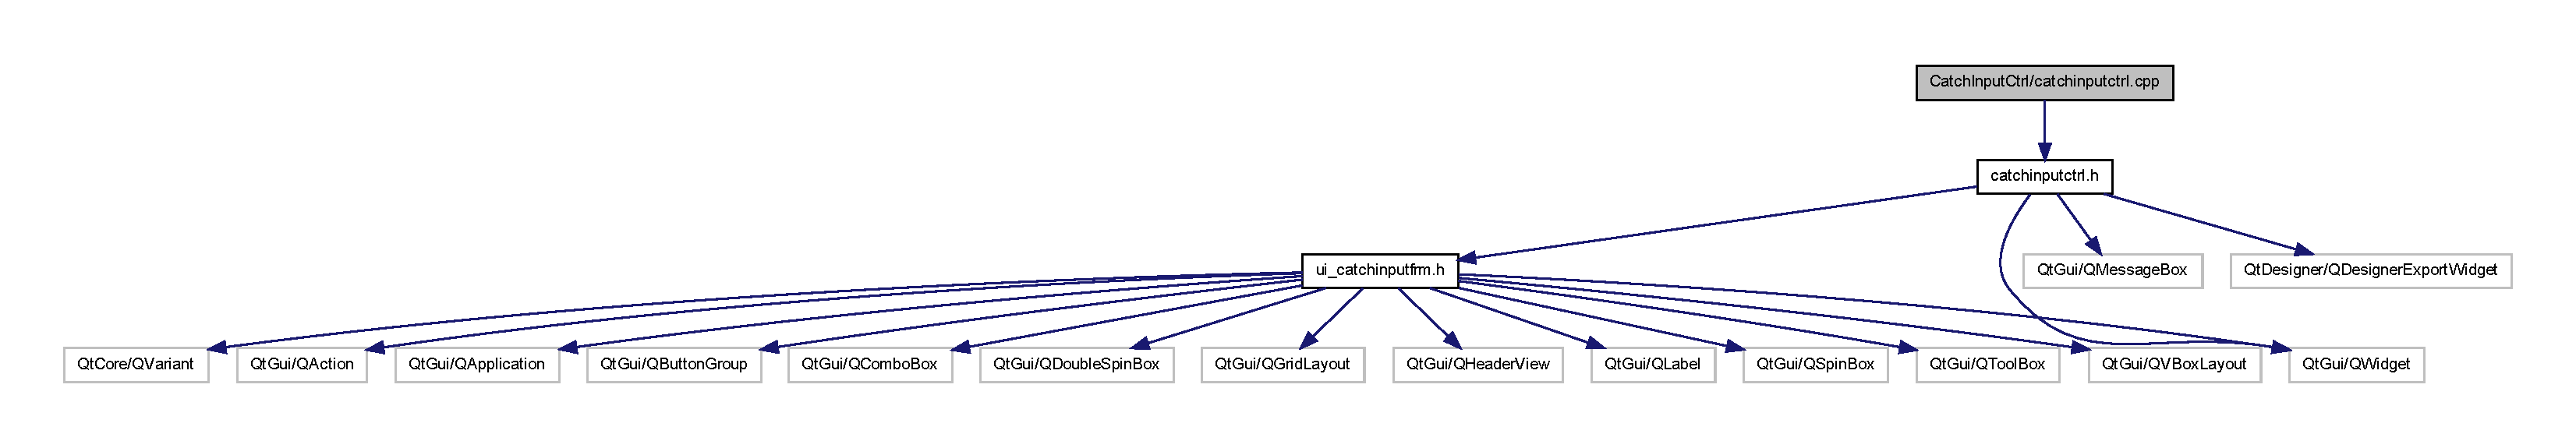
\includegraphics[width=400pt]{catchinputctrl_8cpp__incl}
\end{center}
\end{figure}
\subsection*{Variables}
\begin{DoxyCompactItemize}
\item 
static const char $\ast$ \hyperlink{catchinputctrl_8cpp_a00533981c8e44d54840453cb8f67ef6d}{strWeight}
\item 
static const char $\ast$ \hyperlink{catchinputctrl_8cpp_a40a45457a52d3c046f5b9322005ba5c5}{strUnits}
\item 
static const char $\ast$ \hyperlink{catchinputctrl_8cpp_afd5bf552519d64ed7f33e67905df8e54}{strBoxes}
\end{DoxyCompactItemize}


\subsection{Variable Documentation}
\hypertarget{catchinputctrl_8cpp_afd5bf552519d64ed7f33e67905df8e54}{
\index{catchinputctrl.cpp@{catchinputctrl.cpp}!strBoxes@{strBoxes}}
\index{strBoxes@{strBoxes}!catchinputctrl.cpp@{catchinputctrl.cpp}}
\subsubsection[{strBoxes}]{\setlength{\rightskip}{0pt plus 5cm}const char$\ast$ {\bf strBoxes}\hspace{0.3cm}{\ttfamily  \mbox{[}static\mbox{]}}}}
\label{catchinputctrl_8cpp_afd5bf552519d64ed7f33e67905df8e54}
{\bfseries Initial value:}
\begin{DoxyCode}
 
     QT_TRANSLATE_NOOP("sections", "by Boxes")
\end{DoxyCode}
\hypertarget{catchinputctrl_8cpp_a40a45457a52d3c046f5b9322005ba5c5}{
\index{catchinputctrl.cpp@{catchinputctrl.cpp}!strUnits@{strUnits}}
\index{strUnits@{strUnits}!catchinputctrl.cpp@{catchinputctrl.cpp}}
\subsubsection[{strUnits}]{\setlength{\rightskip}{0pt plus 5cm}const char$\ast$ {\bf strUnits}\hspace{0.3cm}{\ttfamily  \mbox{[}static\mbox{]}}}}
\label{catchinputctrl_8cpp_a40a45457a52d3c046f5b9322005ba5c5}
{\bfseries Initial value:}
\begin{DoxyCode}
 
     QT_TRANSLATE_NOOP("sections", "by Units")
\end{DoxyCode}
\hypertarget{catchinputctrl_8cpp_a00533981c8e44d54840453cb8f67ef6d}{
\index{catchinputctrl.cpp@{catchinputctrl.cpp}!strWeight@{strWeight}}
\index{strWeight@{strWeight}!catchinputctrl.cpp@{catchinputctrl.cpp}}
\subsubsection[{strWeight}]{\setlength{\rightskip}{0pt plus 5cm}const char$\ast$ {\bf strWeight}\hspace{0.3cm}{\ttfamily  \mbox{[}static\mbox{]}}}}
\label{catchinputctrl_8cpp_a00533981c8e44d54840453cb8f67ef6d}
{\bfseries Initial value:}
\begin{DoxyCode}
 
     QT_TRANSLATE_NOOP("sections", "by Weight")
\end{DoxyCode}

\hypertarget{catchinputctrl_8h}{
\section{CatchInputCtrl/catchinputctrl.h File Reference}
\label{catchinputctrl_8h}\index{CatchInputCtrl/catchinputctrl.h@{CatchInputCtrl/catchinputctrl.h}}
}
{\ttfamily \#include \char`\"{}ui\_\-catchinputfrm.h\char`\"{}}\par
{\ttfamily \#include $<$QtGui/QWidget$>$}\par
{\ttfamily \#include $<$QtGui/QMessageBox$>$}\par
{\ttfamily \#include $<$QtDesigner/QDesignerExportWidget$>$}\par
Include dependency graph for catchinputctrl.h:\nopagebreak
\begin{figure}[H]
\begin{center}
\leavevmode
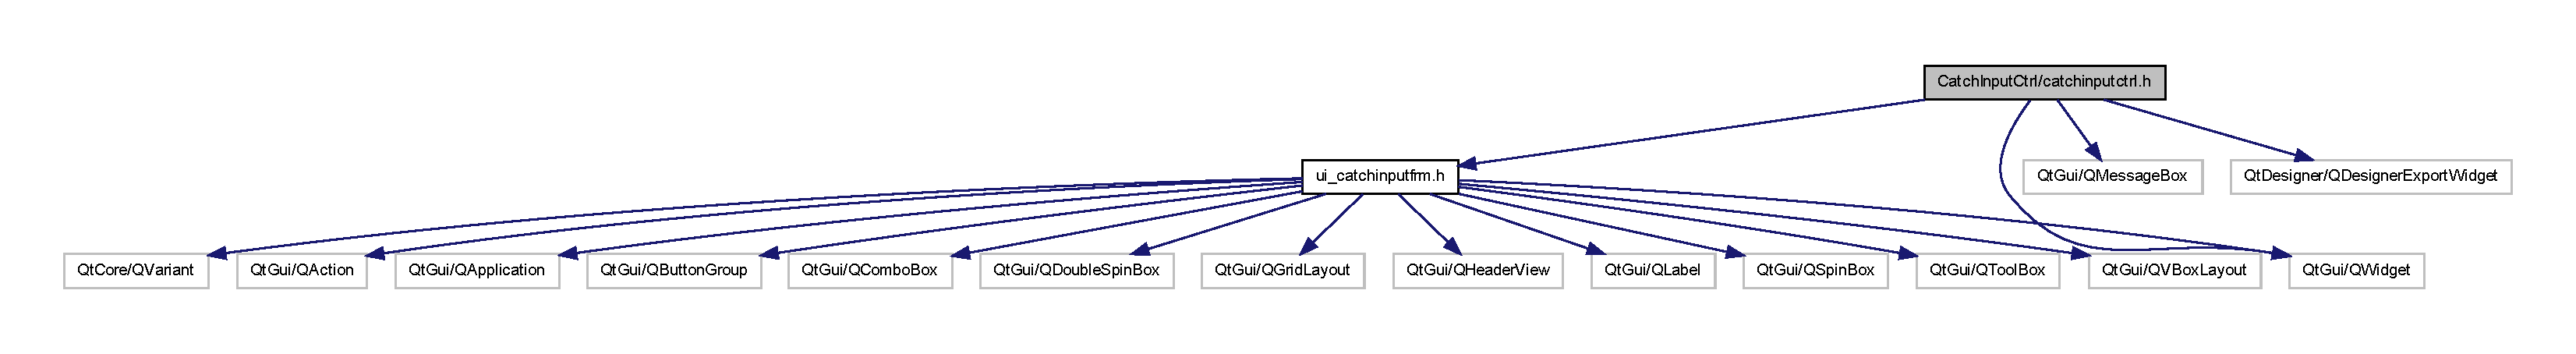
\includegraphics[width=400pt]{catchinputctrl_8h__incl}
\end{center}
\end{figure}
This graph shows which files directly or indirectly include this file:\nopagebreak
\begin{figure}[H]
\begin{center}
\leavevmode
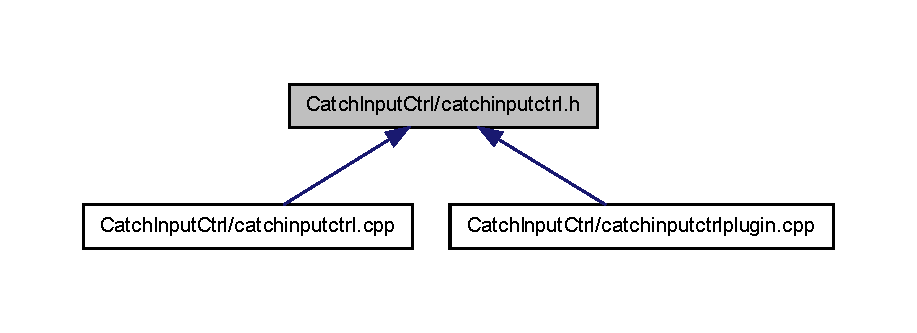
\includegraphics[width=400pt]{catchinputctrl_8h__dep__incl}
\end{center}
\end{figure}
\subsection*{Classes}
\begin{DoxyCompactItemize}
\item 
class \hyperlink{class_catch_input_ctrl}{CatchInputCtrl}
\begin{DoxyCompactList}\small\item\em Custom Input Control class. \item\end{DoxyCompactList}\end{DoxyCompactItemize}

\hypertarget{catchinputctrlplugin_8cpp}{
\section{CatchInputCtrl/catchinputctrlplugin.cpp File Reference}
\label{catchinputctrlplugin_8cpp}\index{CatchInputCtrl/catchinputctrlplugin.cpp@{CatchInputCtrl/catchinputctrlplugin.cpp}}
}
{\ttfamily \#include \char`\"{}catchinputctrl.h\char`\"{}}\par
{\ttfamily \#include $<$QtCore/QtPlugin$>$}\par
{\ttfamily \#include \char`\"{}catchinputctrlplugin.h\char`\"{}}\par
Include dependency graph for catchinputctrlplugin.cpp:\nopagebreak
\begin{figure}[H]
\begin{center}
\leavevmode
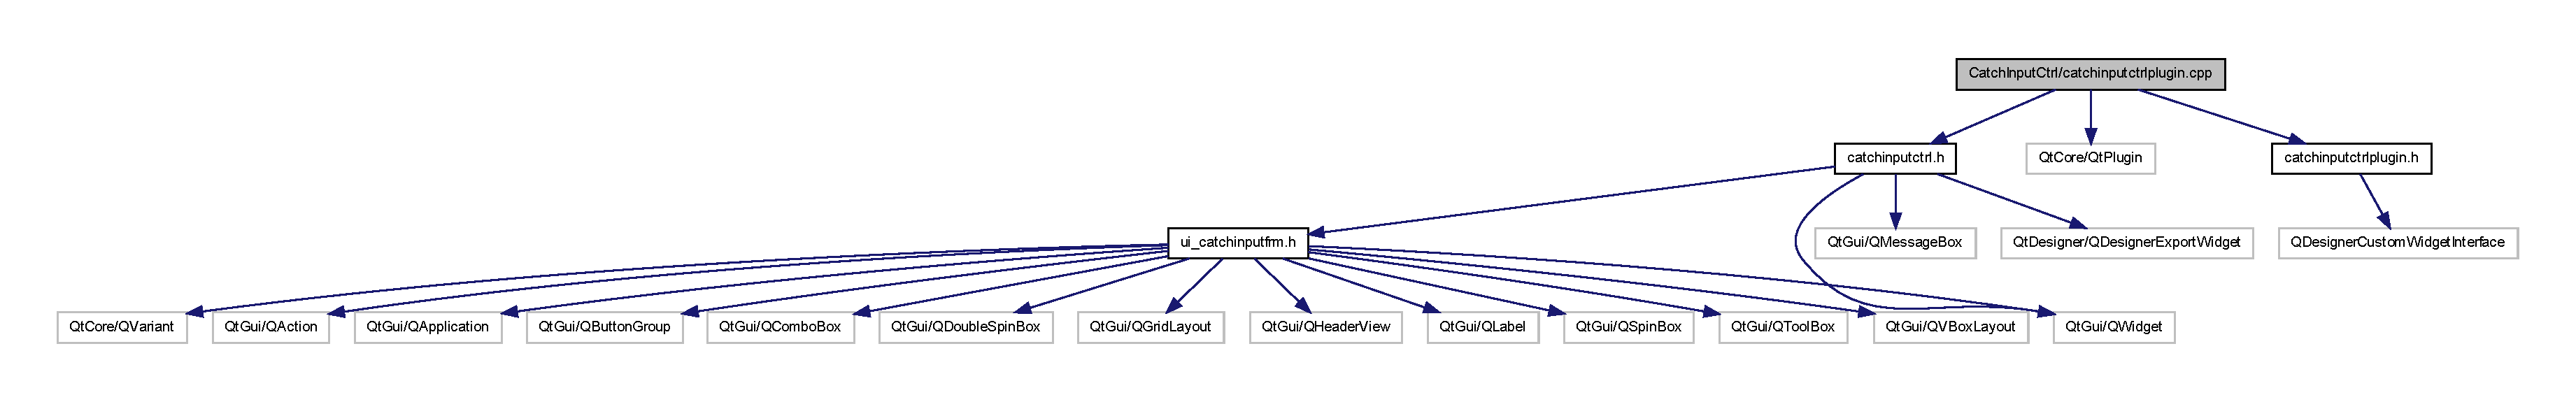
\includegraphics[width=400pt]{catchinputctrlplugin_8cpp__incl}
\end{center}
\end{figure}

\hypertarget{catchinputctrlplugin_8h}{
\section{CatchInputCtrl/catchinputctrlplugin.h File Reference}
\label{catchinputctrlplugin_8h}\index{CatchInputCtrl/catchinputctrlplugin.h@{CatchInputCtrl/catchinputctrlplugin.h}}
}
{\ttfamily \#include $<$QDesignerCustomWidgetInterface$>$}\par
Include dependency graph for catchinputctrlplugin.h:\nopagebreak
\begin{figure}[H]
\begin{center}
\leavevmode
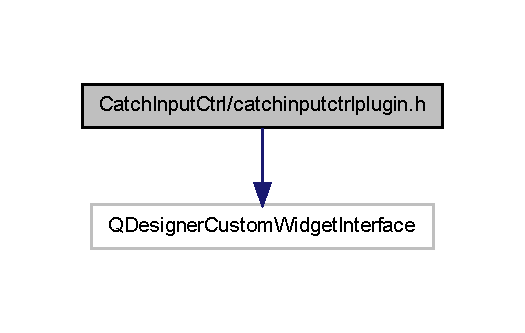
\includegraphics[width=252pt]{catchinputctrlplugin_8h__incl}
\end{center}
\end{figure}
This graph shows which files directly or indirectly include this file:\nopagebreak
\begin{figure}[H]
\begin{center}
\leavevmode
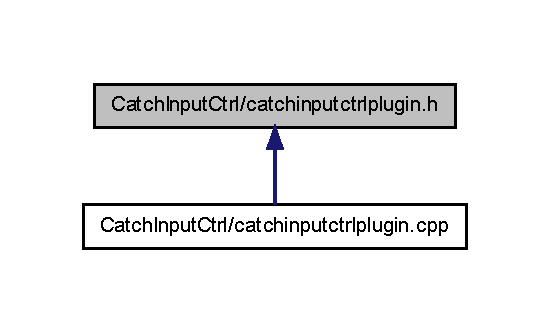
\includegraphics[width=264pt]{catchinputctrlplugin_8h__dep__incl}
\end{center}
\end{figure}
\subsection*{Classes}
\begin{DoxyCompactItemize}
\item 
class \hyperlink{class_catch_input_ctrl_plugin}{CatchInputCtrlPlugin}
\begin{DoxyCompactList}\small\item\em Plugin Class. \item\end{DoxyCompactList}\end{DoxyCompactItemize}

\hypertarget{_debug_2moc__catchinputctrl_8cpp}{
\section{CatchInputCtrl/GeneratedFiles/Debug/moc\_\-catchinputctrl.cpp File Reference}
\label{_debug_2moc__catchinputctrl_8cpp}\index{CatchInputCtrl/GeneratedFiles/Debug/moc\_\-catchinputctrl.cpp@{CatchInputCtrl/GeneratedFiles/Debug/moc\_\-catchinputctrl.cpp}}
}
{\ttfamily \#include \char`\"{}../../catchinputctrl.h\char`\"{}}\par
Include dependency graph for moc\_\-catchinputctrl.cpp:\nopagebreak
\begin{figure}[H]
\begin{center}
\leavevmode
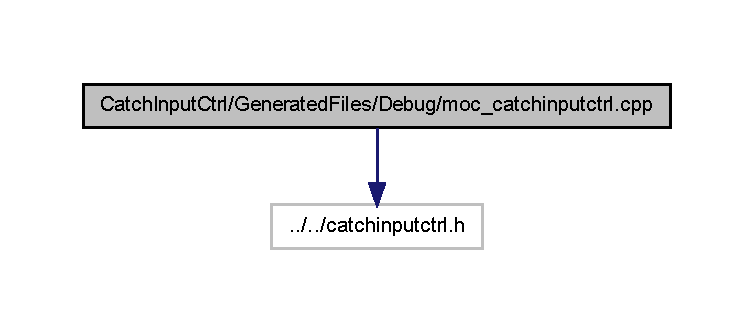
\includegraphics[width=362pt]{_debug_2moc__catchinputctrl_8cpp__incl}
\end{center}
\end{figure}
\subsection*{Variables}
\begin{DoxyCompactItemize}
\item 
static QT\_\-BEGIN\_\-MOC\_\-NAMESPACE const uint \hyperlink{_debug_2moc__catchinputctrl_8cpp_adc228291559383b18fe34686bb4767a8}{qt\_\-meta\_\-data\_\-CatchInputCtrl} \mbox{[}$\,$\mbox{]}
\item 
static const char \hyperlink{_debug_2moc__catchinputctrl_8cpp_acf1775cf9c824beddfd9494bb42d0993}{qt\_\-meta\_\-stringdata\_\-CatchInputCtrl} \mbox{[}$\,$\mbox{]}
\end{DoxyCompactItemize}


\subsection{Variable Documentation}
\hypertarget{_debug_2moc__catchinputctrl_8cpp_adc228291559383b18fe34686bb4767a8}{
\index{Debug/moc\_\-catchinputctrl.cpp@{Debug/moc\_\-catchinputctrl.cpp}!qt\_\-meta\_\-data\_\-CatchInputCtrl@{qt\_\-meta\_\-data\_\-CatchInputCtrl}}
\index{qt\_\-meta\_\-data\_\-CatchInputCtrl@{qt\_\-meta\_\-data\_\-CatchInputCtrl}!Debug/moc_catchinputctrl.cpp@{Debug/moc\_\-catchinputctrl.cpp}}
\subsubsection[{qt\_\-meta\_\-data\_\-CatchInputCtrl}]{\setlength{\rightskip}{0pt plus 5cm}QT\_\-BEGIN\_\-MOC\_\-NAMESPACE const uint {\bf qt\_\-meta\_\-data\_\-CatchInputCtrl}\mbox{[}$\,$\mbox{]}\hspace{0.3cm}{\ttfamily  \mbox{[}static\mbox{]}}}}
\label{_debug_2moc__catchinputctrl_8cpp_adc228291559383b18fe34686bb4767a8}
{\bfseries Initial value:}
\begin{DoxyCode}
 {

 
       5,       
       0,       
       0,    0, 
      10,   14, 
       0,    0, 
       0,    0, 
       0,    0, 
       0,       
       1,       

 
      23,   16,   15,   15, 0x05,

 
      53,   49,   15,   15, 0x08,
      85,   49,   15,   15, 0x08,
     120,   49,   15,   15, 0x08,
     157,   49,   15,   15, 0x08,
     205,  196,   15,   15, 0x08,
     233,  196,   15,   15, 0x08,
     260,  196,   15,   15, 0x08,
     292,  285,   15,   15, 0x08,
     319,   16,   15,   15, 0x08,

       0        
}
\end{DoxyCode}
\hypertarget{_debug_2moc__catchinputctrl_8cpp_acf1775cf9c824beddfd9494bb42d0993}{
\index{Debug/moc\_\-catchinputctrl.cpp@{Debug/moc\_\-catchinputctrl.cpp}!qt\_\-meta\_\-stringdata\_\-CatchInputCtrl@{qt\_\-meta\_\-stringdata\_\-CatchInputCtrl}}
\index{qt\_\-meta\_\-stringdata\_\-CatchInputCtrl@{qt\_\-meta\_\-stringdata\_\-CatchInputCtrl}!Debug/moc_catchinputctrl.cpp@{Debug/moc\_\-catchinputctrl.cpp}}
\subsubsection[{qt\_\-meta\_\-stringdata\_\-CatchInputCtrl}]{\setlength{\rightskip}{0pt plus 5cm}const char {\bf qt\_\-meta\_\-stringdata\_\-CatchInputCtrl}\mbox{[}$\,$\mbox{]}\hspace{0.3cm}{\ttfamily  \mbox{[}static\mbox{]}}}}
\label{_debug_2moc__catchinputctrl_8cpp_acf1775cf9c824beddfd9494bb42d0993}
{\bfseries Initial value:}
\begin{DoxyCode}
 {
    "CatchInputCtrl\0\0bBlock\0blockWidgetsSignals(bool)\0"
    "val\0adjustTotalWeightFromUnits(int)\0"
    "adjustTotalWeightFromUnits(double)\0"
    "adjustTotalWeightFromNoBoxes(double)\0"
    "adjustTotalWeightFromBoxWeight(double)\0"
    "strUnits\0onWeightUnitChange(QString)\0"
    "onUnitsUnitChange(QString)\0"
    "onBoxUnitChange(QString)\0strNew\0"
    "updateWeightLabel(QString)\0"
    "onBlockWidgetsSignals(bool)\0"
}
\end{DoxyCode}

\hypertarget{_release_2moc__catchinputctrl_8cpp}{
\section{CatchInputCtrl/GeneratedFiles/Release/moc\_\-catchinputctrl.cpp File Reference}
\label{_release_2moc__catchinputctrl_8cpp}\index{CatchInputCtrl/GeneratedFiles/Release/moc\_\-catchinputctrl.cpp@{CatchInputCtrl/GeneratedFiles/Release/moc\_\-catchinputctrl.cpp}}
}
{\ttfamily \#include \char`\"{}../../catchinputctrl.h\char`\"{}}\par
Include dependency graph for moc\_\-catchinputctrl.cpp:\nopagebreak
\begin{figure}[H]
\begin{center}
\leavevmode
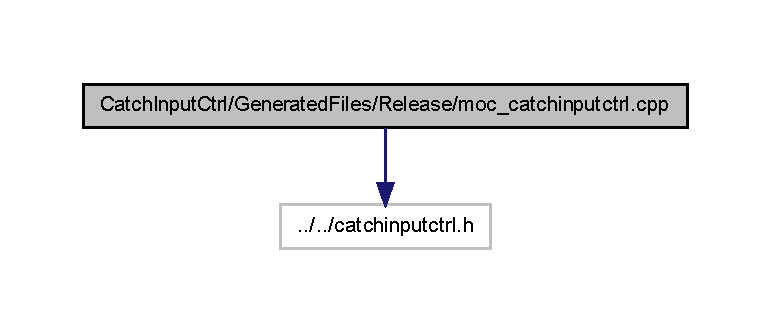
\includegraphics[width=370pt]{_release_2moc__catchinputctrl_8cpp__incl}
\end{center}
\end{figure}
\subsection*{Variables}
\begin{DoxyCompactItemize}
\item 
static QT\_\-BEGIN\_\-MOC\_\-NAMESPACE const uint \hyperlink{_release_2moc__catchinputctrl_8cpp_adc228291559383b18fe34686bb4767a8}{qt\_\-meta\_\-data\_\-CatchInputCtrl} \mbox{[}$\,$\mbox{]}
\item 
static const char \hyperlink{_release_2moc__catchinputctrl_8cpp_acf1775cf9c824beddfd9494bb42d0993}{qt\_\-meta\_\-stringdata\_\-CatchInputCtrl} \mbox{[}$\,$\mbox{]}
\end{DoxyCompactItemize}


\subsection{Variable Documentation}
\hypertarget{_release_2moc__catchinputctrl_8cpp_adc228291559383b18fe34686bb4767a8}{
\index{Release/moc\_\-catchinputctrl.cpp@{Release/moc\_\-catchinputctrl.cpp}!qt\_\-meta\_\-data\_\-CatchInputCtrl@{qt\_\-meta\_\-data\_\-CatchInputCtrl}}
\index{qt\_\-meta\_\-data\_\-CatchInputCtrl@{qt\_\-meta\_\-data\_\-CatchInputCtrl}!Release/moc_catchinputctrl.cpp@{Release/moc\_\-catchinputctrl.cpp}}
\subsubsection[{qt\_\-meta\_\-data\_\-CatchInputCtrl}]{\setlength{\rightskip}{0pt plus 5cm}QT\_\-BEGIN\_\-MOC\_\-NAMESPACE const uint {\bf qt\_\-meta\_\-data\_\-CatchInputCtrl}\mbox{[}$\,$\mbox{]}\hspace{0.3cm}{\ttfamily  \mbox{[}static\mbox{]}}}}
\label{_release_2moc__catchinputctrl_8cpp_adc228291559383b18fe34686bb4767a8}
{\bfseries Initial value:}
\begin{DoxyCode}
 {

 
       5,       
       0,       
       0,    0, 
      10,   14, 
       0,    0, 
       0,    0, 
       0,    0, 
       0,       
       1,       

 
      23,   16,   15,   15, 0x05,

 
      53,   49,   15,   15, 0x08,
      85,   49,   15,   15, 0x08,
     120,   49,   15,   15, 0x08,
     157,   49,   15,   15, 0x08,
     205,  196,   15,   15, 0x08,
     233,  196,   15,   15, 0x08,
     260,  196,   15,   15, 0x08,
     292,  285,   15,   15, 0x08,
     319,   16,   15,   15, 0x08,

       0        
}
\end{DoxyCode}
\hypertarget{_release_2moc__catchinputctrl_8cpp_acf1775cf9c824beddfd9494bb42d0993}{
\index{Release/moc\_\-catchinputctrl.cpp@{Release/moc\_\-catchinputctrl.cpp}!qt\_\-meta\_\-stringdata\_\-CatchInputCtrl@{qt\_\-meta\_\-stringdata\_\-CatchInputCtrl}}
\index{qt\_\-meta\_\-stringdata\_\-CatchInputCtrl@{qt\_\-meta\_\-stringdata\_\-CatchInputCtrl}!Release/moc_catchinputctrl.cpp@{Release/moc\_\-catchinputctrl.cpp}}
\subsubsection[{qt\_\-meta\_\-stringdata\_\-CatchInputCtrl}]{\setlength{\rightskip}{0pt plus 5cm}const char {\bf qt\_\-meta\_\-stringdata\_\-CatchInputCtrl}\mbox{[}$\,$\mbox{]}\hspace{0.3cm}{\ttfamily  \mbox{[}static\mbox{]}}}}
\label{_release_2moc__catchinputctrl_8cpp_acf1775cf9c824beddfd9494bb42d0993}
{\bfseries Initial value:}
\begin{DoxyCode}
 {
    "CatchInputCtrl\0\0bBlock\0blockWidgetsSignals(bool)\0"
    "val\0adjustTotalWeightFromUnits(int)\0"
    "adjustTotalWeightFromUnits(double)\0"
    "adjustTotalWeightFromNoBoxes(double)\0"
    "adjustTotalWeightFromBoxWeight(double)\0"
    "strUnits\0onWeightUnitChange(QString)\0"
    "onUnitsUnitChange(QString)\0"
    "onBoxUnitChange(QString)\0strNew\0"
    "updateWeightLabel(QString)\0"
    "onBlockWidgetsSignals(bool)\0"
}
\end{DoxyCode}

\hypertarget{_debug_2moc__catchinputctrlplugin_8cpp}{
\section{CatchInputCtrl/GeneratedFiles/Debug/moc\_\-catchinputctrlplugin.cpp File Reference}
\label{_debug_2moc__catchinputctrlplugin_8cpp}\index{CatchInputCtrl/GeneratedFiles/Debug/moc\_\-catchinputctrlplugin.cpp@{CatchInputCtrl/GeneratedFiles/Debug/moc\_\-catchinputctrlplugin.cpp}}
}
{\ttfamily \#include \char`\"{}../../catchinputctrlplugin.h\char`\"{}}\par
Include dependency graph for moc\_\-catchinputctrlplugin.cpp:\nopagebreak
\begin{figure}[H]
\begin{center}
\leavevmode
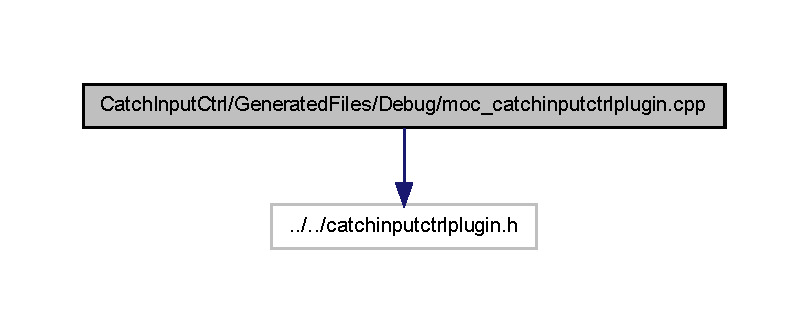
\includegraphics[width=388pt]{_debug_2moc__catchinputctrlplugin_8cpp__incl}
\end{center}
\end{figure}
\subsection*{Variables}
\begin{DoxyCompactItemize}
\item 
static QT\_\-BEGIN\_\-MOC\_\-NAMESPACE const uint \hyperlink{_debug_2moc__catchinputctrlplugin_8cpp_ae1450eb58cc46f57b9e54156aad90412}{qt\_\-meta\_\-data\_\-CatchInputCtrlPlugin} \mbox{[}$\,$\mbox{]}
\item 
static const char \hyperlink{_debug_2moc__catchinputctrlplugin_8cpp_aa0a06662a5e1e82077e8a0768910258f}{qt\_\-meta\_\-stringdata\_\-CatchInputCtrlPlugin} \mbox{[}$\,$\mbox{]}
\end{DoxyCompactItemize}


\subsection{Variable Documentation}
\hypertarget{_debug_2moc__catchinputctrlplugin_8cpp_ae1450eb58cc46f57b9e54156aad90412}{
\index{Debug/moc\_\-catchinputctrlplugin.cpp@{Debug/moc\_\-catchinputctrlplugin.cpp}!qt\_\-meta\_\-data\_\-CatchInputCtrlPlugin@{qt\_\-meta\_\-data\_\-CatchInputCtrlPlugin}}
\index{qt\_\-meta\_\-data\_\-CatchInputCtrlPlugin@{qt\_\-meta\_\-data\_\-CatchInputCtrlPlugin}!Debug/moc_catchinputctrlplugin.cpp@{Debug/moc\_\-catchinputctrlplugin.cpp}}
\subsubsection[{qt\_\-meta\_\-data\_\-CatchInputCtrlPlugin}]{\setlength{\rightskip}{0pt plus 5cm}QT\_\-BEGIN\_\-MOC\_\-NAMESPACE const uint {\bf qt\_\-meta\_\-data\_\-CatchInputCtrlPlugin}\mbox{[}$\,$\mbox{]}\hspace{0.3cm}{\ttfamily  \mbox{[}static\mbox{]}}}}
\label{_debug_2moc__catchinputctrlplugin_8cpp_ae1450eb58cc46f57b9e54156aad90412}
{\bfseries Initial value:}
\begin{DoxyCode}
 {

 
       5,       
       0,       
       0,    0, 
       0,    0, 
       0,    0, 
       0,    0, 
       0,    0, 
       0,       
       0,       

       0        
}
\end{DoxyCode}
\hypertarget{_debug_2moc__catchinputctrlplugin_8cpp_aa0a06662a5e1e82077e8a0768910258f}{
\index{Debug/moc\_\-catchinputctrlplugin.cpp@{Debug/moc\_\-catchinputctrlplugin.cpp}!qt\_\-meta\_\-stringdata\_\-CatchInputCtrlPlugin@{qt\_\-meta\_\-stringdata\_\-CatchInputCtrlPlugin}}
\index{qt\_\-meta\_\-stringdata\_\-CatchInputCtrlPlugin@{qt\_\-meta\_\-stringdata\_\-CatchInputCtrlPlugin}!Debug/moc_catchinputctrlplugin.cpp@{Debug/moc\_\-catchinputctrlplugin.cpp}}
\subsubsection[{qt\_\-meta\_\-stringdata\_\-CatchInputCtrlPlugin}]{\setlength{\rightskip}{0pt plus 5cm}const char {\bf qt\_\-meta\_\-stringdata\_\-CatchInputCtrlPlugin}\mbox{[}$\,$\mbox{]}\hspace{0.3cm}{\ttfamily  \mbox{[}static\mbox{]}}}}
\label{_debug_2moc__catchinputctrlplugin_8cpp_aa0a06662a5e1e82077e8a0768910258f}
{\bfseries Initial value:}
\begin{DoxyCode}
 {
    "CatchInputCtrlPlugin\0"
}
\end{DoxyCode}

\hypertarget{_release_2moc__catchinputctrlplugin_8cpp}{
\section{CatchInputCtrl/GeneratedFiles/Release/moc\_\-catchinputctrlplugin.cpp File Reference}
\label{_release_2moc__catchinputctrlplugin_8cpp}\index{CatchInputCtrl/GeneratedFiles/Release/moc\_\-catchinputctrlplugin.cpp@{CatchInputCtrl/GeneratedFiles/Release/moc\_\-catchinputctrlplugin.cpp}}
}
{\ttfamily \#include \char`\"{}../../catchinputctrlplugin.h\char`\"{}}\par
Include dependency graph for moc\_\-catchinputctrlplugin.cpp:\nopagebreak
\begin{figure}[H]
\begin{center}
\leavevmode
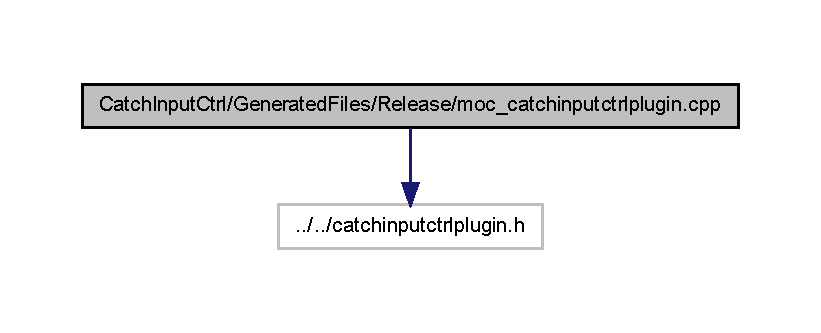
\includegraphics[width=394pt]{_release_2moc__catchinputctrlplugin_8cpp__incl}
\end{center}
\end{figure}
\subsection*{Variables}
\begin{DoxyCompactItemize}
\item 
static QT\_\-BEGIN\_\-MOC\_\-NAMESPACE const uint \hyperlink{_release_2moc__catchinputctrlplugin_8cpp_ae1450eb58cc46f57b9e54156aad90412}{qt\_\-meta\_\-data\_\-CatchInputCtrlPlugin} \mbox{[}$\,$\mbox{]}
\item 
static const char \hyperlink{_release_2moc__catchinputctrlplugin_8cpp_aa0a06662a5e1e82077e8a0768910258f}{qt\_\-meta\_\-stringdata\_\-CatchInputCtrlPlugin} \mbox{[}$\,$\mbox{]}
\end{DoxyCompactItemize}


\subsection{Variable Documentation}
\hypertarget{_release_2moc__catchinputctrlplugin_8cpp_ae1450eb58cc46f57b9e54156aad90412}{
\index{Release/moc\_\-catchinputctrlplugin.cpp@{Release/moc\_\-catchinputctrlplugin.cpp}!qt\_\-meta\_\-data\_\-CatchInputCtrlPlugin@{qt\_\-meta\_\-data\_\-CatchInputCtrlPlugin}}
\index{qt\_\-meta\_\-data\_\-CatchInputCtrlPlugin@{qt\_\-meta\_\-data\_\-CatchInputCtrlPlugin}!Release/moc_catchinputctrlplugin.cpp@{Release/moc\_\-catchinputctrlplugin.cpp}}
\subsubsection[{qt\_\-meta\_\-data\_\-CatchInputCtrlPlugin}]{\setlength{\rightskip}{0pt plus 5cm}QT\_\-BEGIN\_\-MOC\_\-NAMESPACE const uint {\bf qt\_\-meta\_\-data\_\-CatchInputCtrlPlugin}\mbox{[}$\,$\mbox{]}\hspace{0.3cm}{\ttfamily  \mbox{[}static\mbox{]}}}}
\label{_release_2moc__catchinputctrlplugin_8cpp_ae1450eb58cc46f57b9e54156aad90412}
{\bfseries Initial value:}
\begin{DoxyCode}
 {

 
       5,       
       0,       
       0,    0, 
       0,    0, 
       0,    0, 
       0,    0, 
       0,    0, 
       0,       
       0,       

       0        
}
\end{DoxyCode}
\hypertarget{_release_2moc__catchinputctrlplugin_8cpp_aa0a06662a5e1e82077e8a0768910258f}{
\index{Release/moc\_\-catchinputctrlplugin.cpp@{Release/moc\_\-catchinputctrlplugin.cpp}!qt\_\-meta\_\-stringdata\_\-CatchInputCtrlPlugin@{qt\_\-meta\_\-stringdata\_\-CatchInputCtrlPlugin}}
\index{qt\_\-meta\_\-stringdata\_\-CatchInputCtrlPlugin@{qt\_\-meta\_\-stringdata\_\-CatchInputCtrlPlugin}!Release/moc_catchinputctrlplugin.cpp@{Release/moc\_\-catchinputctrlplugin.cpp}}
\subsubsection[{qt\_\-meta\_\-stringdata\_\-CatchInputCtrlPlugin}]{\setlength{\rightskip}{0pt plus 5cm}const char {\bf qt\_\-meta\_\-stringdata\_\-CatchInputCtrlPlugin}\mbox{[}$\,$\mbox{]}\hspace{0.3cm}{\ttfamily  \mbox{[}static\mbox{]}}}}
\label{_release_2moc__catchinputctrlplugin_8cpp_aa0a06662a5e1e82077e8a0768910258f}
{\bfseries Initial value:}
\begin{DoxyCode}
 {
    "CatchInputCtrlPlugin\0"
}
\end{DoxyCode}

\hypertarget{qrc___catch_input_ctrl_8cpp}{
\section{CatchInputCtrl/GeneratedFiles/qrc\_\-CatchInputCtrl.cpp File Reference}
\label{qrc___catch_input_ctrl_8cpp}\index{CatchInputCtrl/GeneratedFiles/qrc\_\-CatchInputCtrl.cpp@{CatchInputCtrl/GeneratedFiles/qrc\_\-CatchInputCtrl.cpp}}
}
{\ttfamily \#include $<$QtCore/qglobal.h$>$}\par
Include dependency graph for qrc\_\-CatchInputCtrl.cpp:\nopagebreak
\begin{figure}[H]
\begin{center}
\leavevmode
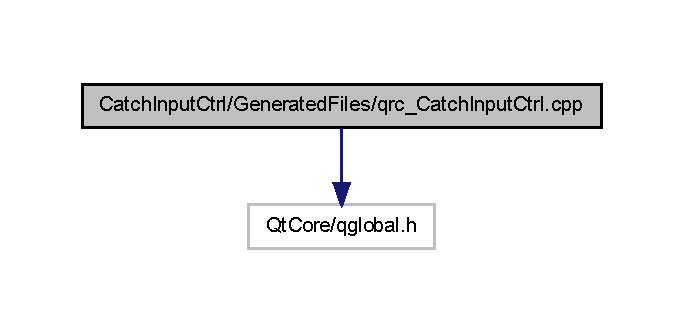
\includegraphics[width=328pt]{qrc___catch_input_ctrl_8cpp__incl}
\end{center}
\end{figure}
\subsection*{Functions}
\begin{DoxyCompactItemize}
\item 
QT\_\-BEGIN\_\-NAMESPACE Q\_\-CORE\_\-EXPORT bool \hyperlink{qrc___catch_input_ctrl_8cpp_ab3bec3d1e679084be46edc41e4c91bc1}{qRegisterResourceData} (int, const unsigned char $\ast$, const unsigned char $\ast$, const unsigned char $\ast$)
\item 
Q\_\-CORE\_\-EXPORT bool \hyperlink{qrc___catch_input_ctrl_8cpp_ad65f8bca8010dd1fd135a28a085c6d03}{qUnregisterResourceData} (int, const unsigned char $\ast$, const unsigned char $\ast$, const unsigned char $\ast$)
\item 
QT\_\-END\_\-NAMESPACE int QT\_\-MANGLE\_\-NAMESPACE() \hyperlink{qrc___catch_input_ctrl_8cpp_aa7ab37edf4823074979eb7e50a07d7bb}{qInitResources\_\-CatchInputCtrl} ()
\item 
int QT\_\-MANGLE\_\-NAMESPACE() \hyperlink{qrc___catch_input_ctrl_8cpp_a12873cf0001e7317520e0319203ef317}{qCleanupResources\_\-CatchInputCtrl} ()
\end{DoxyCompactItemize}
\subsection*{Variables}
\begin{DoxyCompactItemize}
\item 
static const unsigned char \hyperlink{qrc___catch_input_ctrl_8cpp_a67a985282ed24629b630f624b668842b}{qt\_\-resource\_\-data} \mbox{[}$\,$\mbox{]}
\item 
static const unsigned char \hyperlink{qrc___catch_input_ctrl_8cpp_a7931167bf9d7e883e4194a60d031e431}{qt\_\-resource\_\-name} \mbox{[}$\,$\mbox{]}
\item 
static const unsigned char \hyperlink{qrc___catch_input_ctrl_8cpp_a37a83d7da2ee18badcd100d79aac64d4}{qt\_\-resource\_\-struct} \mbox{[}$\,$\mbox{]}
\end{DoxyCompactItemize}


\subsection{Function Documentation}
\hypertarget{qrc___catch_input_ctrl_8cpp_a12873cf0001e7317520e0319203ef317}{
\index{qrc\_\-CatchInputCtrl.cpp@{qrc\_\-CatchInputCtrl.cpp}!qCleanupResources\_\-CatchInputCtrl@{qCleanupResources\_\-CatchInputCtrl}}
\index{qCleanupResources\_\-CatchInputCtrl@{qCleanupResources\_\-CatchInputCtrl}!qrc_CatchInputCtrl.cpp@{qrc\_\-CatchInputCtrl.cpp}}
\subsubsection[{qCleanupResources\_\-CatchInputCtrl}]{\setlength{\rightskip}{0pt plus 5cm}int QT\_\-MANGLE\_\-NAMESPACE() qCleanupResources\_\-CatchInputCtrl (
\begin{DoxyParamCaption}
{}
\end{DoxyParamCaption}
)}}
\label{qrc___catch_input_ctrl_8cpp_a12873cf0001e7317520e0319203ef317}


Here is the call graph for this function:\nopagebreak
\begin{figure}[H]
\begin{center}
\leavevmode
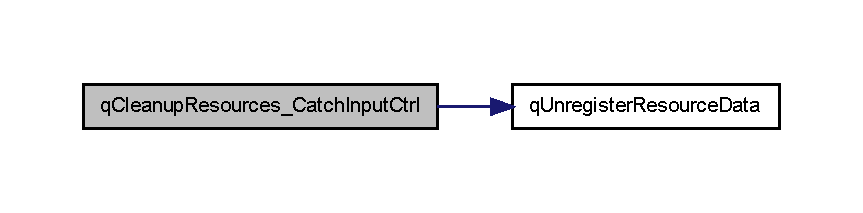
\includegraphics[width=400pt]{qrc___catch_input_ctrl_8cpp_a12873cf0001e7317520e0319203ef317_cgraph}
\end{center}
\end{figure}


\hypertarget{qrc___catch_input_ctrl_8cpp_aa7ab37edf4823074979eb7e50a07d7bb}{
\index{qrc\_\-CatchInputCtrl.cpp@{qrc\_\-CatchInputCtrl.cpp}!qInitResources\_\-CatchInputCtrl@{qInitResources\_\-CatchInputCtrl}}
\index{qInitResources\_\-CatchInputCtrl@{qInitResources\_\-CatchInputCtrl}!qrc_CatchInputCtrl.cpp@{qrc\_\-CatchInputCtrl.cpp}}
\subsubsection[{qInitResources\_\-CatchInputCtrl}]{\setlength{\rightskip}{0pt plus 5cm}QT\_\-END\_\-NAMESPACE int QT\_\-MANGLE\_\-NAMESPACE() qInitResources\_\-CatchInputCtrl (
\begin{DoxyParamCaption}
{}
\end{DoxyParamCaption}
)}}
\label{qrc___catch_input_ctrl_8cpp_aa7ab37edf4823074979eb7e50a07d7bb}


Here is the call graph for this function:\nopagebreak
\begin{figure}[H]
\begin{center}
\leavevmode
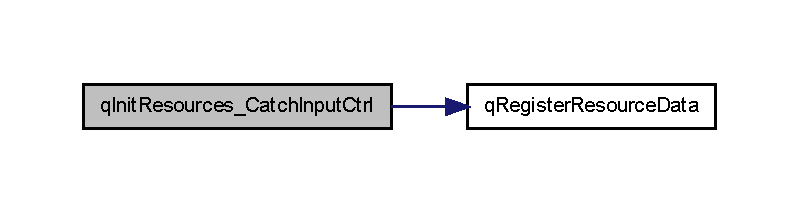
\includegraphics[width=384pt]{qrc___catch_input_ctrl_8cpp_aa7ab37edf4823074979eb7e50a07d7bb_cgraph}
\end{center}
\end{figure}


\hypertarget{qrc___catch_input_ctrl_8cpp_ab3bec3d1e679084be46edc41e4c91bc1}{
\index{qrc\_\-CatchInputCtrl.cpp@{qrc\_\-CatchInputCtrl.cpp}!qRegisterResourceData@{qRegisterResourceData}}
\index{qRegisterResourceData@{qRegisterResourceData}!qrc_CatchInputCtrl.cpp@{qrc\_\-CatchInputCtrl.cpp}}
\subsubsection[{qRegisterResourceData}]{\setlength{\rightskip}{0pt plus 5cm}QT\_\-BEGIN\_\-NAMESPACE Q\_\-CORE\_\-EXPORT bool qRegisterResourceData (
\begin{DoxyParamCaption}
\item[{int}]{, }
\item[{const unsigned char $\ast$}]{, }
\item[{const unsigned char $\ast$}]{, }
\item[{const unsigned char $\ast$}]{}
\end{DoxyParamCaption}
)}}
\label{qrc___catch_input_ctrl_8cpp_ab3bec3d1e679084be46edc41e4c91bc1}


Here is the caller graph for this function:\nopagebreak
\begin{figure}[H]
\begin{center}
\leavevmode
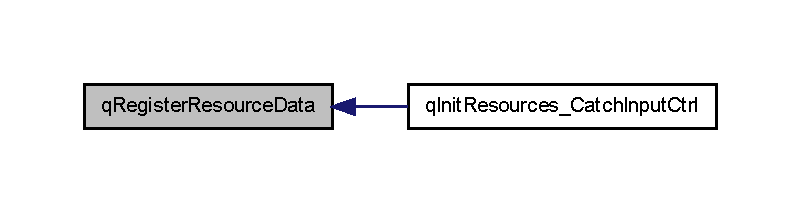
\includegraphics[width=384pt]{qrc___catch_input_ctrl_8cpp_ab3bec3d1e679084be46edc41e4c91bc1_icgraph}
\end{center}
\end{figure}


\hypertarget{qrc___catch_input_ctrl_8cpp_ad65f8bca8010dd1fd135a28a085c6d03}{
\index{qrc\_\-CatchInputCtrl.cpp@{qrc\_\-CatchInputCtrl.cpp}!qUnregisterResourceData@{qUnregisterResourceData}}
\index{qUnregisterResourceData@{qUnregisterResourceData}!qrc_CatchInputCtrl.cpp@{qrc\_\-CatchInputCtrl.cpp}}
\subsubsection[{qUnregisterResourceData}]{\setlength{\rightskip}{0pt plus 5cm}Q\_\-CORE\_\-EXPORT bool qUnregisterResourceData (
\begin{DoxyParamCaption}
\item[{int}]{, }
\item[{const unsigned char $\ast$}]{, }
\item[{const unsigned char $\ast$}]{, }
\item[{const unsigned char $\ast$}]{}
\end{DoxyParamCaption}
)}}
\label{qrc___catch_input_ctrl_8cpp_ad65f8bca8010dd1fd135a28a085c6d03}


Here is the caller graph for this function:\nopagebreak
\begin{figure}[H]
\begin{center}
\leavevmode
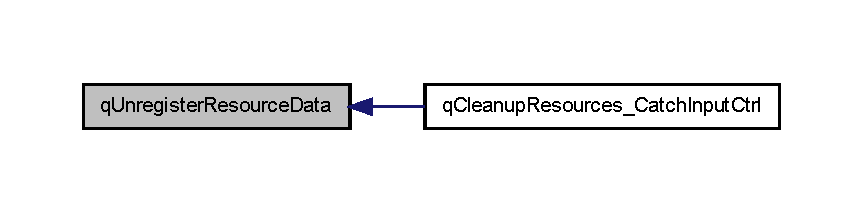
\includegraphics[width=400pt]{qrc___catch_input_ctrl_8cpp_ad65f8bca8010dd1fd135a28a085c6d03_icgraph}
\end{center}
\end{figure}




\subsection{Variable Documentation}
\hypertarget{qrc___catch_input_ctrl_8cpp_a67a985282ed24629b630f624b668842b}{
\index{qrc\_\-CatchInputCtrl.cpp@{qrc\_\-CatchInputCtrl.cpp}!qt\_\-resource\_\-data@{qt\_\-resource\_\-data}}
\index{qt\_\-resource\_\-data@{qt\_\-resource\_\-data}!qrc_CatchInputCtrl.cpp@{qrc\_\-CatchInputCtrl.cpp}}
\subsubsection[{qt\_\-resource\_\-data}]{\setlength{\rightskip}{0pt plus 5cm}const unsigned char {\bf qt\_\-resource\_\-data}\mbox{[}$\,$\mbox{]}\hspace{0.3cm}{\ttfamily  \mbox{[}static\mbox{]}}}}
\label{qrc___catch_input_ctrl_8cpp_a67a985282ed24629b630f624b668842b}
\hypertarget{qrc___catch_input_ctrl_8cpp_a7931167bf9d7e883e4194a60d031e431}{
\index{qrc\_\-CatchInputCtrl.cpp@{qrc\_\-CatchInputCtrl.cpp}!qt\_\-resource\_\-name@{qt\_\-resource\_\-name}}
\index{qt\_\-resource\_\-name@{qt\_\-resource\_\-name}!qrc_CatchInputCtrl.cpp@{qrc\_\-CatchInputCtrl.cpp}}
\subsubsection[{qt\_\-resource\_\-name}]{\setlength{\rightskip}{0pt plus 5cm}const unsigned char {\bf qt\_\-resource\_\-name}\mbox{[}$\,$\mbox{]}\hspace{0.3cm}{\ttfamily  \mbox{[}static\mbox{]}}}}
\label{qrc___catch_input_ctrl_8cpp_a7931167bf9d7e883e4194a60d031e431}
{\bfseries Initial value:}
\begin{DoxyCode}
 {
  
  0x0,0x4,
  0x0,0x6,0xd0,0x98,
  0x0,0x66,
  0x0,0x69,0x0,0x73,0x0,0x68,
  
}
\end{DoxyCode}
\hypertarget{qrc___catch_input_ctrl_8cpp_a37a83d7da2ee18badcd100d79aac64d4}{
\index{qrc\_\-CatchInputCtrl.cpp@{qrc\_\-CatchInputCtrl.cpp}!qt\_\-resource\_\-struct@{qt\_\-resource\_\-struct}}
\index{qt\_\-resource\_\-struct@{qt\_\-resource\_\-struct}!qrc_CatchInputCtrl.cpp@{qrc\_\-CatchInputCtrl.cpp}}
\subsubsection[{qt\_\-resource\_\-struct}]{\setlength{\rightskip}{0pt plus 5cm}const unsigned char {\bf qt\_\-resource\_\-struct}\mbox{[}$\,$\mbox{]}\hspace{0.3cm}{\ttfamily  \mbox{[}static\mbox{]}}}}
\label{qrc___catch_input_ctrl_8cpp_a37a83d7da2ee18badcd100d79aac64d4}
{\bfseries Initial value:}
\begin{DoxyCode}
 {
  
  0x0,0x0,0x0,0x0,0x0,0x2,0x0,0x0,0x0,0x1,0x0,0x0,0x0,0x1,
  
  0x0,0x0,0x0,0x0,0x0,0x0,0x0,0x0,0x0,0x1,0x0,0x0,0x0,0x0,

}
\end{DoxyCode}

\hypertarget{ui__catchinputfrm_8h}{
\section{CatchInputCtrl/GeneratedFiles/ui\_\-catchinputfrm.h File Reference}
\label{ui__catchinputfrm_8h}\index{CatchInputCtrl/GeneratedFiles/ui\_\-catchinputfrm.h@{CatchInputCtrl/GeneratedFiles/ui\_\-catchinputfrm.h}}
}
{\ttfamily \#include $<$QtCore/QVariant$>$}\par
{\ttfamily \#include $<$QtGui/QAction$>$}\par
{\ttfamily \#include $<$QtGui/QApplication$>$}\par
{\ttfamily \#include $<$QtGui/QButtonGroup$>$}\par
{\ttfamily \#include $<$QtGui/QComboBox$>$}\par
{\ttfamily \#include $<$QtGui/QDoubleSpinBox$>$}\par
{\ttfamily \#include $<$QtGui/QGridLayout$>$}\par
{\ttfamily \#include $<$QtGui/QHeaderView$>$}\par
{\ttfamily \#include $<$QtGui/QLabel$>$}\par
{\ttfamily \#include $<$QtGui/QSpinBox$>$}\par
{\ttfamily \#include $<$QtGui/QToolBox$>$}\par
{\ttfamily \#include $<$QtGui/QVBoxLayout$>$}\par
{\ttfamily \#include $<$QtGui/QWidget$>$}\par
Include dependency graph for ui\_\-catchinputfrm.h:\nopagebreak
\begin{figure}[H]
\begin{center}
\leavevmode
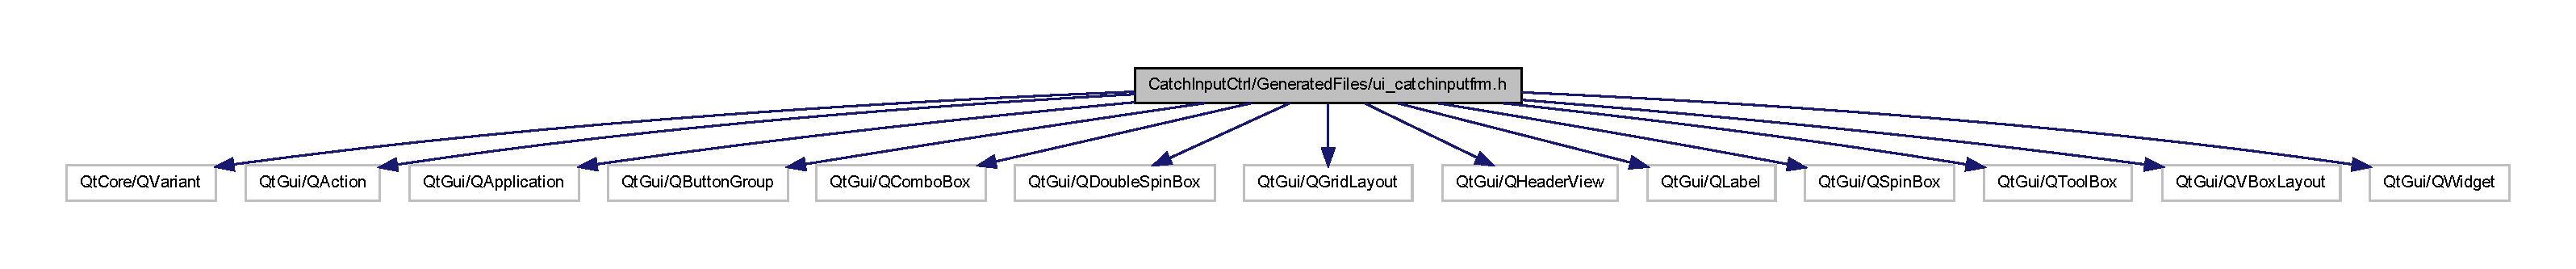
\includegraphics[width=400pt]{ui__catchinputfrm_8h__incl}
\end{center}
\end{figure}
This graph shows which files directly or indirectly include this file:\nopagebreak
\begin{figure}[H]
\begin{center}
\leavevmode
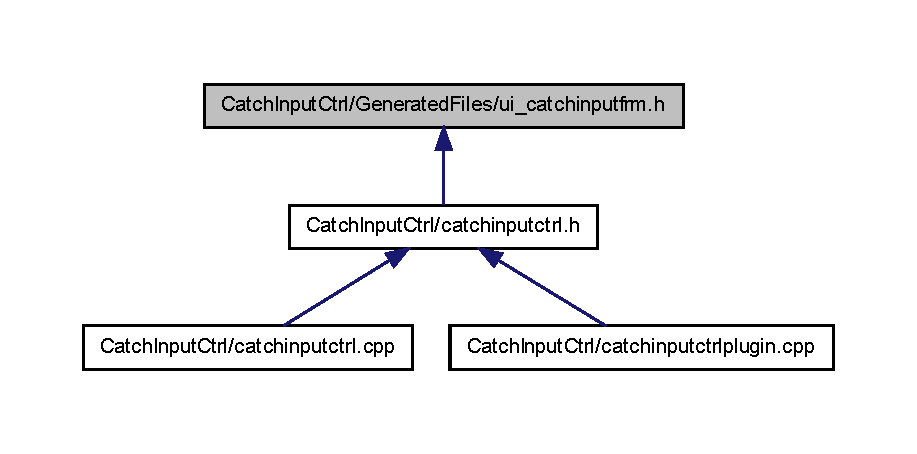
\includegraphics[width=400pt]{ui__catchinputfrm_8h__dep__incl}
\end{center}
\end{figure}
\subsection*{Classes}
\begin{DoxyCompactItemize}
\item 
class \hyperlink{class_ui___catch_input_ctrl}{Ui\_\-CatchInputCtrl}
\item 
class \hyperlink{class_ui_1_1_catch_input_ctrl}{Ui::CatchInputCtrl}
\end{DoxyCompactItemize}
\subsection*{Namespaces}
\begin{DoxyCompactItemize}
\item 
namespace \hyperlink{namespace_ui}{Ui}
\end{DoxyCompactItemize}

\printindex
\end{document}
